\vbox{

    \appendix

    \centering
    {\Large\bf
        Supplementary Material: \\
        \ourslong
        \par}
}
\vspace{10pt}


\renewcommand{\thesection}{\Alph{section}}
\renewcommand{\thesubsection}{\thesection.\arabic{subsection}}
\renewcommand{\thetable}{S\arabic{table}}
\renewcommand{\thefigure}{S\arabic{figure}}
\renewcommand{\theequation}{S\arabic{equation}}
\setcounter{figure}{0}
\setcounter{table}{0}
\setcounter{equation}{0}

In the appendix, we provide detailed implementation details in \S\ref{sec:impl_details}, elaborate on evaluation protocols and additional results in \S\ref{sec:evaluation_protos}, and discuss the understanding of position embeddings in ViT in \S\ref{sec:understanding}. Lastly, we discuss the limitations of this work and propose a few avenues for future work in \S\ref{sec:limitation}.


\section{Implementation Details}
\label{sec:impl_details}

\subsection{Denosing with Neural Fields}

Recall that we decompose the output feature map from a pre-trained ViT into three components: $\mathbf{y}\approx \mathcal{F}(\mathcal{A}) + \mathcal{G} + \mathbf{h}(\mathbf{y})$, where $\mathcal{F}$ is a feature semantic field, $\mathcal{G}$ is an artifact field, and $\vb{h}$ is a residual predictor. We describe their implementation details below.

\paragraph{Neural field $\mathcal{F}$.} To facilitate efficient learning, we use InstantNGP \cite{muller2022instant}, a type of compact and fast coordinate network, parameterized by learnable multi-level hash grids $\mathcal{H}$ and a lightweight MLP $\phi(\cdot)$, to learn $\mathcal{F}$. It takes as input a normalized 2D coordinate $(i, j)$, within the range of [0, 1], and outputs its corresponding feature vector, \ie, $\mathcal{F}(i, j) = \phi\left(\mathcal{H}(i, j)\right)$. We refer readers to \cite{muller2022instant} for a more detailed understanding of the learnable hash grids.  In our implementation, we use a hash encoding resolution that spans from $2^4$ to $2^{10}$ with 16 levels. Each hash entry has a channel size of 8. The maximum number of hash entries of each resolution is $2^{20}$. For the lightweight MLP, we use a two-layer \texttt{Linear-ReLu-Linear} structure. The hidden dimension of this MLP is half the size of the output feature dimension, which corresponds to the feature dimension of the ViT being studied (\eg, 768 for a ViT-\textit{base} and 1024 for a ViT-\textit{large}).

%##################################################################################################
\begin{figure}
    \centering
    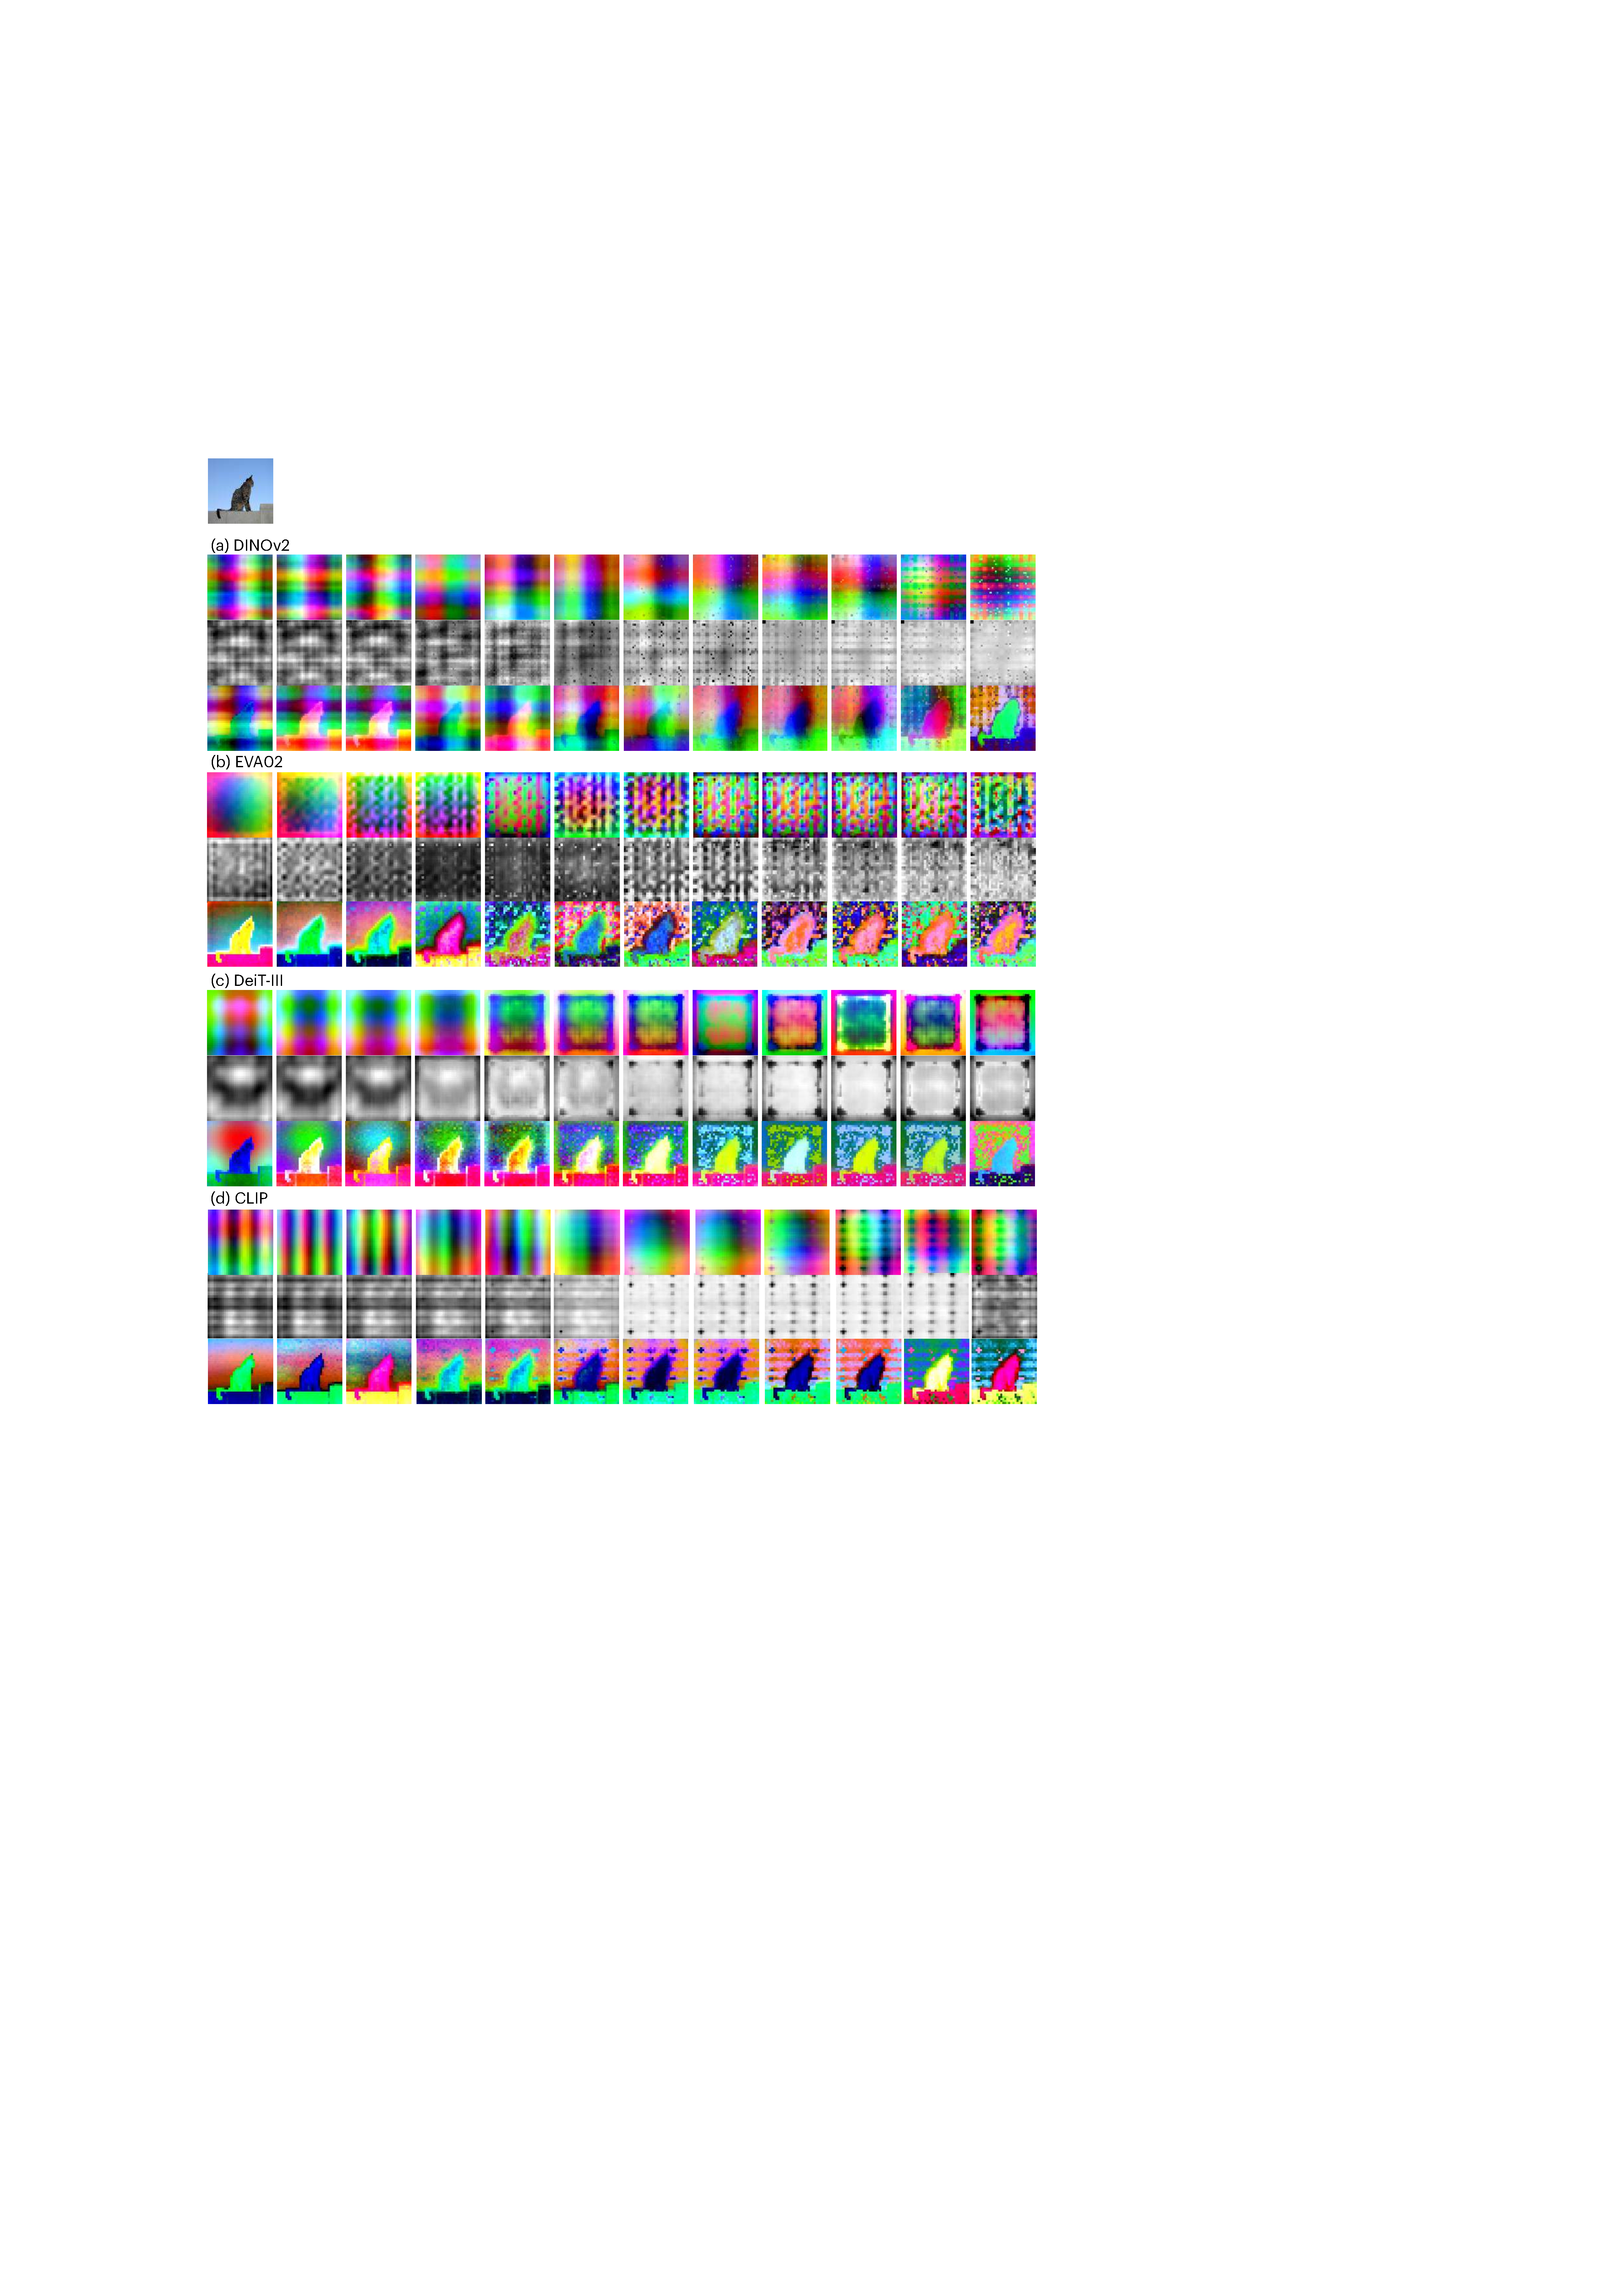
\includegraphics[width=\linewidth]{figures/multilayer_strong.pdf}
    \caption{
        \textbf{Feature map visualizations: positional embeddings (PE) and a cat image in different ViTs.} We visualize the feature maps across different layers (1 to 12) of various pre-trained ViT-base models, displayed sequentially from left to right. For each panel, the top row shows the feature maps generated by inputting a zero tensor, highlighting the influence of PE alone. The middle row presents the feature norm of the PE feature map. The bottom row presents the feature map for a sample cat image, allowing for a comparison that reveals visual correlations between the artifacts in general image feature maps and the PE feature map.
    }
    \label{fig:strong_multilayer}
\end{figure}
%##################################################################################################

\paragraph{Artifact field $\mathcal{G}$.} For all experiments, we use a 2D learnable feature map of size $C\times K \times K$ to learn the input-independent noise, where $C$ corresponds to the feature dimension of the studied ViT, and $K$ is the spatial size. We compute $K$ by $(H - P) / S + 1$, where $H$ is the height\&width of input images (which we resize to be square), $P$ is the patch size, and $S$ is the stride size used in the model. To accommodate ViTs with different patch sizes, we set $H$ to 518 for those trained with a patch size of 14, and 512 for ViTs with a patch size of 16, resulting in $K$ values of 37 and 32, respectively. Note that this feature map, $\mathcal{G}$, can be bilinearly interpolated to fit any arbitrary image resolution. We specifically choose these $K$ values to minimize the need for run-time interpolation during training, thus improving denoising efficiency.

\paragraph{Residual predictor $\mathbf{h}$.} The residual predictor is structured as a 3-layer MLP with \texttt{ReLU} activation after the hidden layers. The hidden dimension is set to be one-quarter of the channel dimension of the ViT being studied.


\paragraph{Optimization.} In our implementation, we extract  $N=768$ views (crops) from each image, applying random augmentations, which include random flipping with a probability of 0.5, and random resizing and cropping, where the size of the crop is scaled between 0.1 to 0.5 of the original image size and the aspect ratio is maintained between 3/4 and 4/3. For understanding how the number of views used for training affects the DVT's performance, please refer to \cref{fig:scaling} in the main text (our default setting is $N=768$).

The coefficients in our loss function ((\cref{eq:recon}) of the main text) are set as $\alpha=0.1$ and $\beta=0.02$. We use Adam optimizer, with a learning rate of 0.01 and a \texttt{LinearLR} decay strategy. Our models are trained for 20,000 iterations. Each iteration will process 2048 randomly sampled pixels from the pre-extracted feature maps. Note that due to the efficient implementation of $\mathcal{F}$ and the pre-extraction of patch features, our denoising typically takes about 100-160 seconds to finish (including the feature extraction time). This rapid optimization process allows us to easily amortize the denoising cost with parallel computes, thereby ensuring the practicality and applicability of our method in various scenarios.

We use the same hyperparameters for all experiments without any specific tuning. See \cref{fig:per_img_dinov2,fig:per_img_clip,fig:per_img_deit,fig:per_img_eva,fig:per_img_mae,fig:per_img_dino,fig:per_img_register} for visualizations of some examples of our per-image denoising output.


\subsection{Generalizable Denoiser}

%##################################################################################################
\begin{figure}
    \centering
    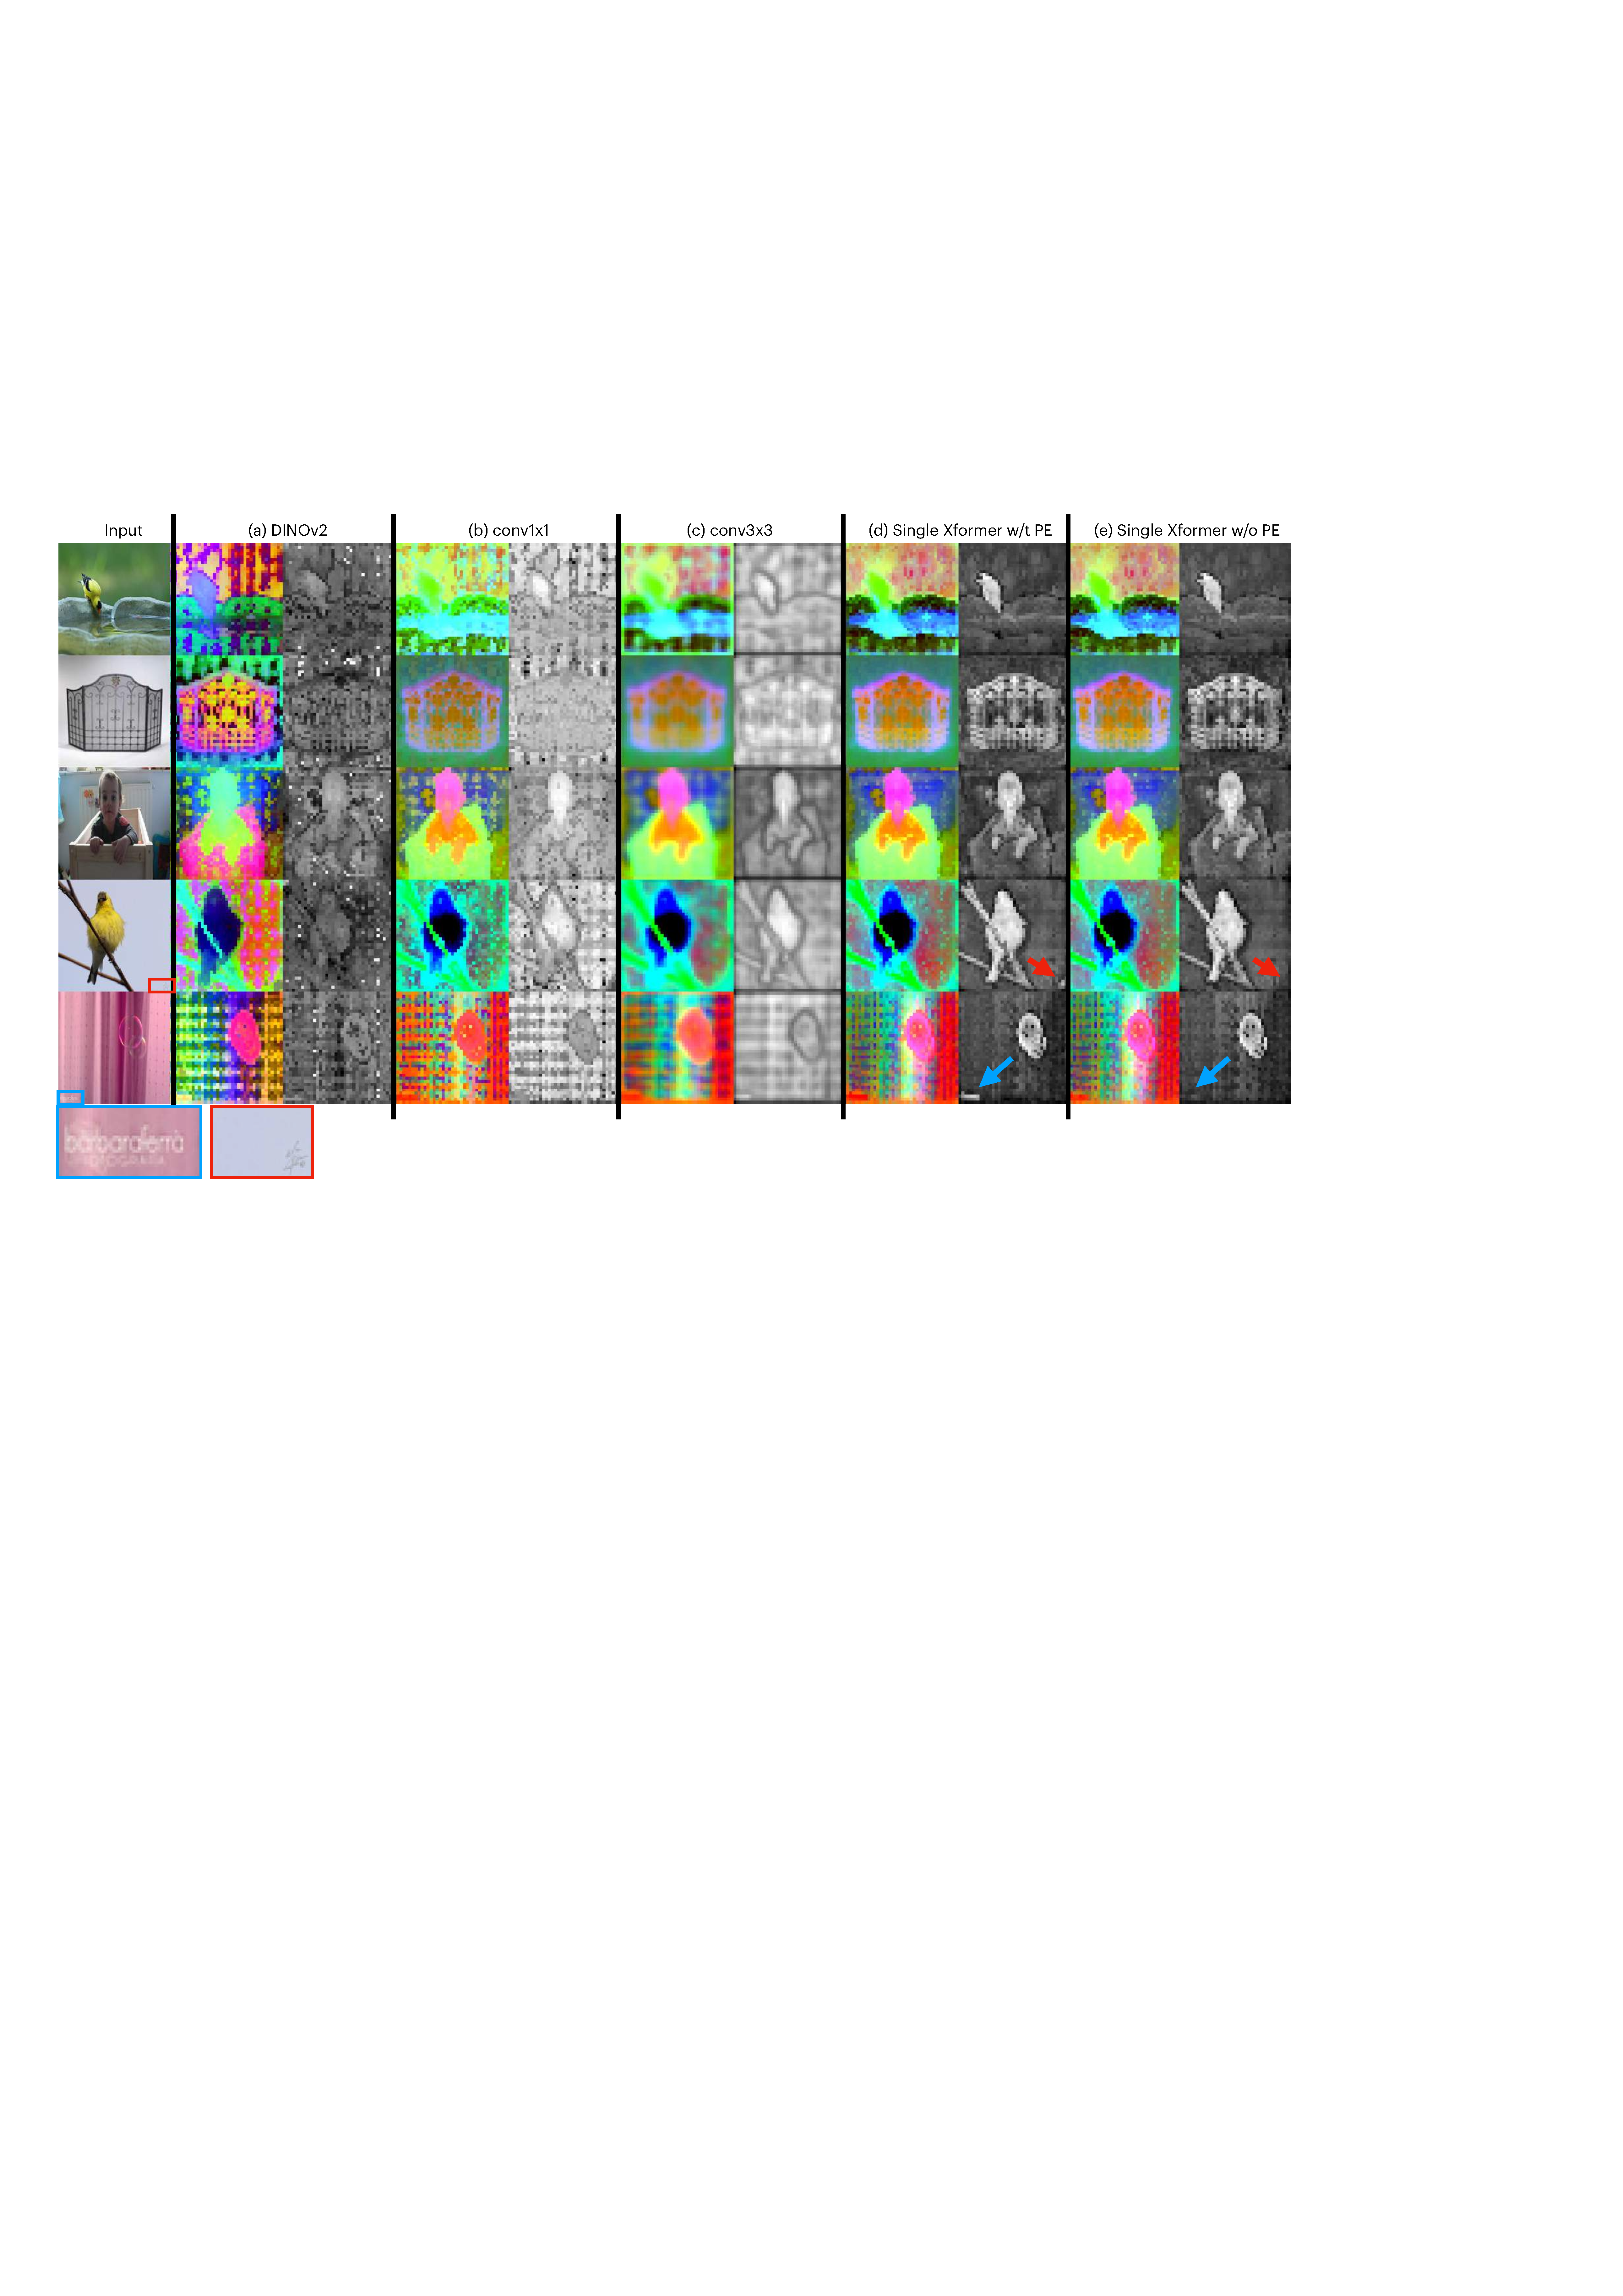
\includegraphics[width=1\linewidth]{figures/arch_ablation.pdf}
    \caption{\textbf{Qualitative comparison of different denoiser architecture designs}. Convolution-based denoisers typically do not yield good performance (b, c). We empirically find that the denoiser with learnable new positional embeddings (PE) is sensitive to subtle details (see the blue and red rectangles and arrows). ``Xformer'': Transformer block. }
    \label{fig:arch_ablation}
\end{figure}
%##################################################################################################
\paragraph{Optimization.} To train the denoiser, we optimize the loss function defined in \cref{eq:gen_loss} of the main text. Note that our approach does not necessitate re-training ViTs; instead, it only optimizes the smaller denoisier network, which constitutes only 8\% of the original model's size. The denoiser is trained for 10 epochs with a batch size of 64, using the \texttt{AdamW} optimizer with a learning rate of $2e-$4 and a cosine learning rate scheduler. The denoiser training typically takes about 2 hours on 8 GPUs.



\subsection{ViT Models}
\paragraph{Model identifiers.} We provide the \texttt{timm} model identifiers of the ViTs studied in this paper in \cref{tab:model_id}. For experiments with large input image sizes (\eg using the 512-sized images as input to a model trained with 224-image resolution), we always resize the position embeddings using bicubic interpolation to accommodate the increased size.
%##################################################################################################
\begin{table*}
    \centering
    \small
    \caption{\textbf{\texttt{timm} model identifiers}}
    \tablestyle{3.5pt}{1.2}
    \footnotesize
    \begin{tabular}{l | y{185}}
        Model                            & Model identifier                                                \\
        \shline
        DINOv2 \cite{oquab2023dinov2}    & \texttt{vit\_base\_patch14\_dinov2.lvd142m}                     \\
        Register \cite{darcet2023vision} & \texttt{vit\_base\_patch14\_reg4\_dinov2.lvd142m}               \\
        DINO \cite{caron2021emerging}    & \texttt{vit\_base\_patch16\_224.dino}                           \\
        MAE \cite{he2022masked}          & \texttt{vit\_base\_patch16\_224.mae}                            \\
        EVA02 \cite{fang2023eva}         & \texttt{eva02\_base\_patch16\_clip\_224.merged2b}               \\
        CLIP \cite{radford2021learning}  & \texttt{vit\_base\_patch16\_clip\_384.laion2b\_ft\_in12k\_in1k} \\
        DeiT-III \cite{touvron2022deit}  & \texttt{deit3\_base\_patch16\_224.fb\_in1k}                     \\
    \end{tabular}
    \label{tab:model_id}
\end{table*}
%##################################################################################################

\subsection{Correlation}
In the main text, we mention the correlation between artifacts and their positions in images without a detailed context, which we now provide. Our focus is on quantifying the correlation between different features and their positions within an image. To analyze this correlation, we employ the maximal information coefficient (MIC), a metric originally used for measuring the strength of linear or nonlinear associations between two scalar variables. To adapt MIC for our purpose, we compute the association between high-dimensional features $\mathbf{f}$ and their positions. We calculate this by taking the maximal MIC across all channels of $\mathbf{f}$ and averaging the MICs of the coordinates $x$ and $y$.
\begin{equation}
    \frac{\max_{c \in \mathcal{C}}{\text{MIC}(\mathbf{f}(x, :), x)} + \max_{c \in \mathcal{C}}{\text{MIC}(\mathbf{f}(:, y), y)}}{2},
\end{equation}
where $\mathbf{f}(x, :)$ denotes the feature vector on the $x$-coordinate, $\mathbf{f}(:, y)$ at the $y$-coordinate, and $\mathcal{C}$ is the channel size of $\mathbf{f}$. For hyperparameters of scalar MIC, we set $B=(H \times W)^{0.6}$:
\begin{equation}
    \text{MIC}(\mathbf{X}; \mathbf{Y}) = \max_{|\mathbf{X}| |\mathbf{Y}| < B} \frac{I[\mathbf{X}; \mathbf{Y}]}{\log_2{(\min{(|\mathbf{X}|, |\mathbf{Y}|}))}},
\end{equation}
where $I[\mathbf{X}; \mathbf{Y}]$ denotes the mutual information between two random variables $\mathbf{X}$ and $\mathbf{Y}$. We compute this metric from 100 randomly selected samples from the ImageNet dataset.

Our analysis includes a comparison of the MIC values for the decomposed noise map, the original noisy ViT features, and the denoised, artifact-free features. The results, presented in \cref{tab:correlation} of the main paper, reveal that the decomposed noise map exhibits the highest correlation with image positions. The noisy features, which are entangled with noise artifacts originating from the position embeddings, display the second highest positional correlation. In contrast, the noise-free features denoised by our method show the lowest correlation with positions, demonstrating the effectiveness of our decomposition approach in removing such artifacts.

\subsection{Feature Qualitative Results}

\paragraph{Algorithms producing mild artifacts.}
We additionally visualize the features for algorithms with weak artifacts in \cref{fig:weak-artif}.
We empirically observe that ViTs trained using both MAE and DINO exhibit very few visible artifacts in their feature (center column). \cref{fig:per_img_dino,fig:per_img_mae} shows additional visualizations of the decomposed noise map and the learned residual terms of DINO and MAE, respectively. We note that decomposed noise maps from these two models typically manifest low-frequency patterns and the residual terms do not yield pronounced patterns.


%##################################################################################################
\begin{figure}[t]
    \centering
    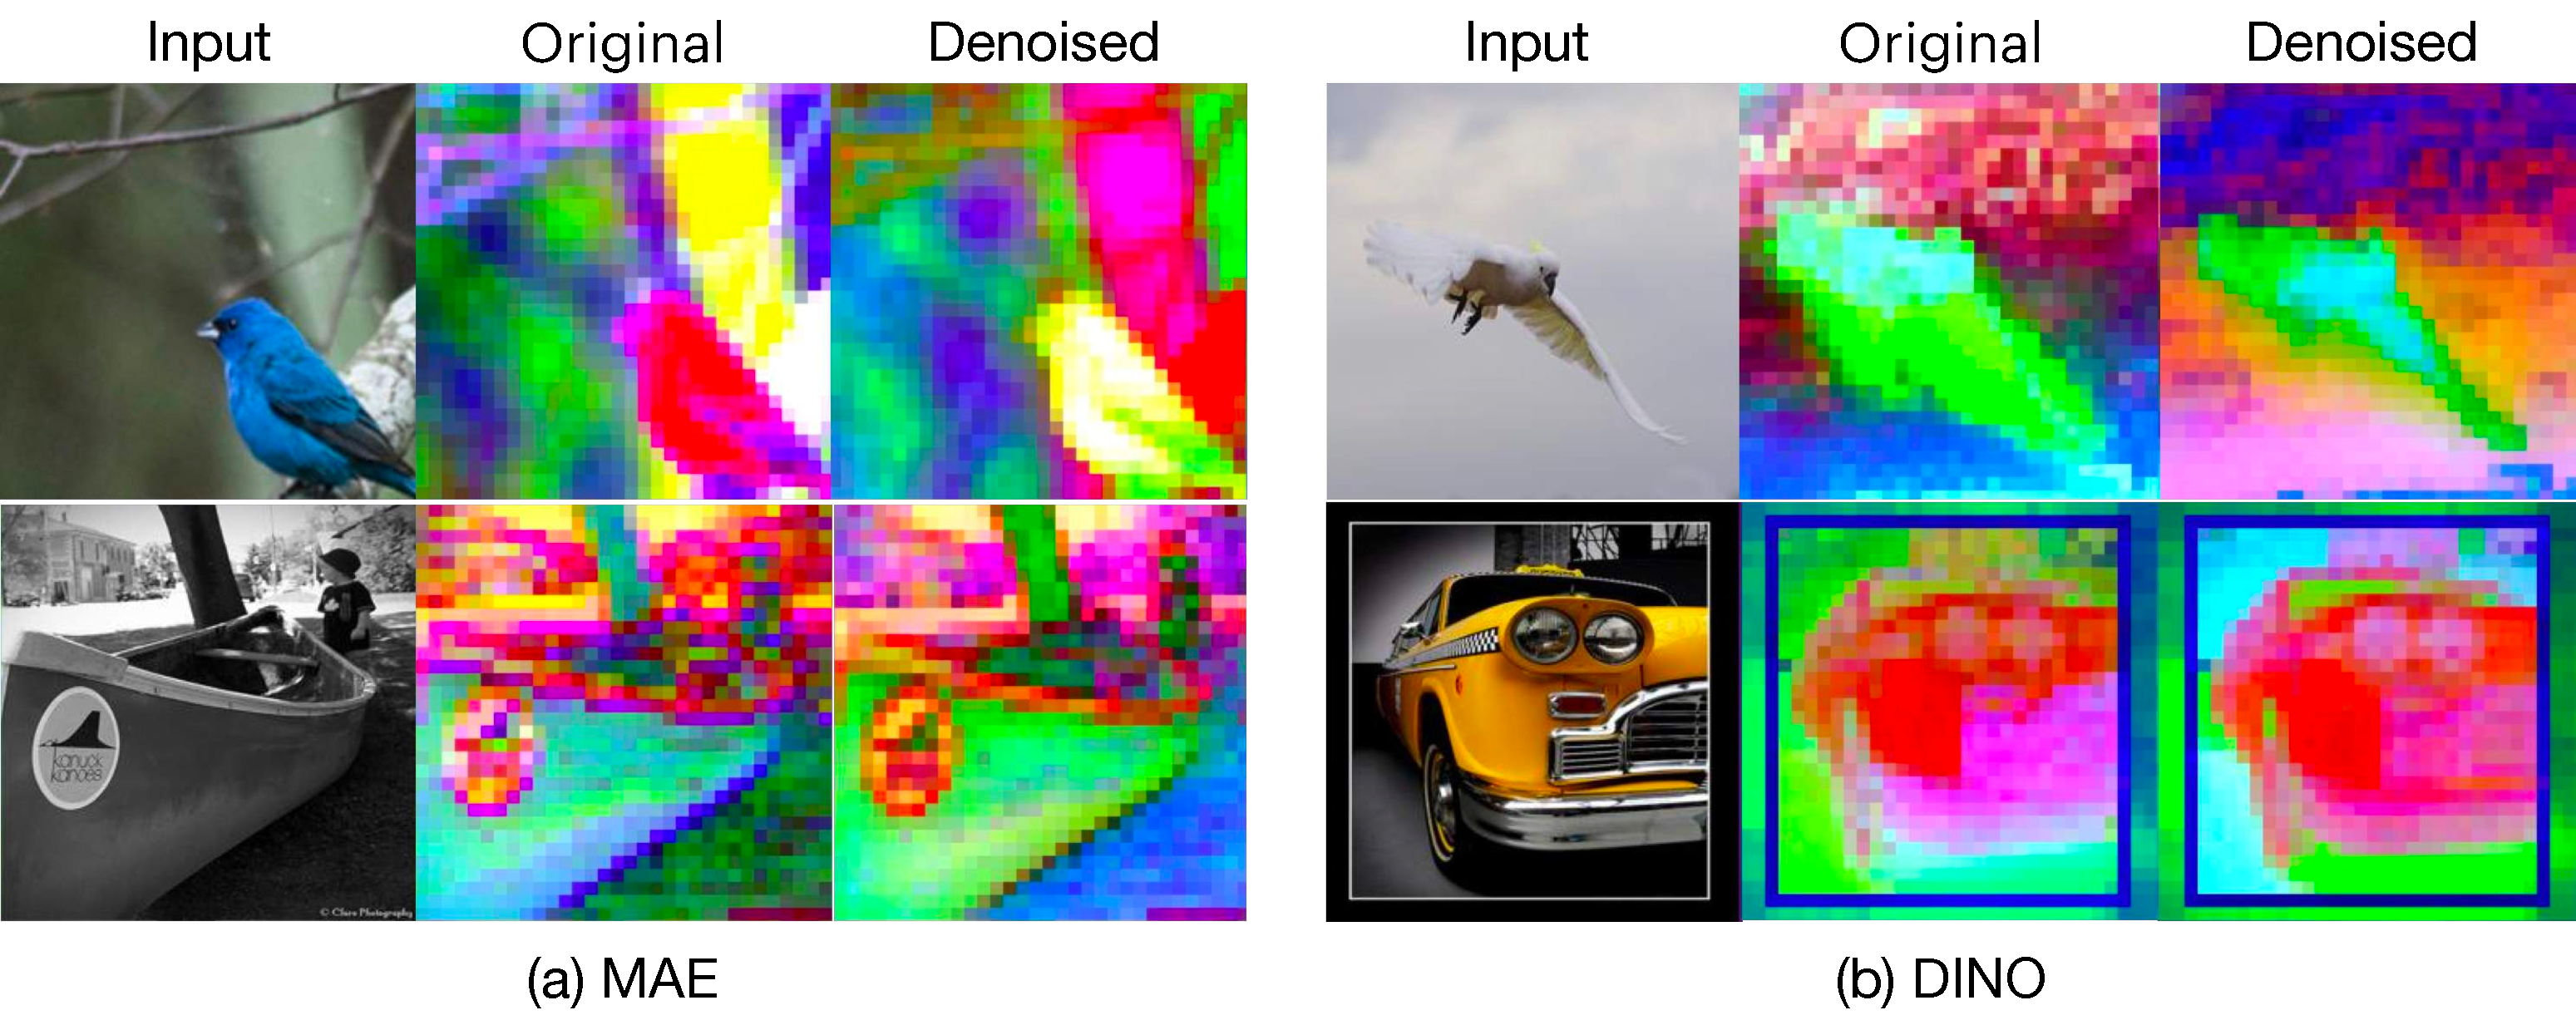
\includegraphics[width=0.85\linewidth]{figures/weak-artifact-vis.pdf}
    \caption{
    \textbf{Features from Weak Artifact Algorithms.}
    }
    \label{fig:weak-artif}

\end{figure}
\paragraph{Additional visualizations.}
%##################################################################################################
Additional visualizations of the feature maps at all layers of ViT models are shown in \cref{fig:strong_multilayer}. Observe that the artifact is present in almost all layers of the models. See \cref{fig:per_img_dinov2,fig:per_img_clip,fig:per_img_deit,fig:per_img_eva,fig:per_img_mae,fig:per_img_dino,fig:per_img_register} for more visualizations.


\section{Evaluation Protocols}
\label{sec:evaluation_protos}

We introduce our evaluation protocols here, mostly following \cite{oquab2023dinov2}. We have released our code, checkpoints, and logs for reproducibility at \url{https://jiawei-yang.github.io/DenoisingViT/}.

\paragraph{Semantic Segmentation.} We use a linear evaluation setting. In detail, we extract the final feature maps from the frozen backbone and pass them through the denoisers if there are any. Following this, feature maps are resized back to their original resolution. Then, a single learnable linear layer is trained to predict the semantic segmentation from these resized feature maps. The training and testing image resolutions are $518\times 518$, following \cite{oquab2023dinov2}. We train this linear head for $40,000$ iterations for both VOC and ADE20k datasets. We report the mean intersection over union (mIoU) metric for all experiments.

\paragraph{Depth estimation.} We extract the final feature maps from the frozen backbone and pass them through the denoisers, if applicable. Then, we follow \cite{oquab2023dinov2} to append the \texttt{cls} token to every patch token to enrich feature representations. We bilinearly upsample these features by a factor of 4 and train a linear layer using classification loss to divide the prediction into 256 uniformly distributed bins. Unlike \cite{oquab2023dinov2}, we slightly decrease the learning rate from 1e-4 to 5e-3, as we find that this modification improves most of the methods, including baselines, in our early experiments.
We report our results on the commonly used metrics: AbsRel (absolute relative error $\abs{d^{*} - d}/d$) and $\delta_1$ (percentage of pixels where $\max(d^{*}/d,~ d/d^{*}) < 1.25$).


\paragraph{Object detection.} To evaluate the object detection task, we utilize the ViTDet detector \cite{li2022exploring} to infer object bounding boxes based on feature maps extracted either from original ViTs or denoisers. The detection framework is FasterRCNN \cite{ren2015faster}. The input image resolution for training and testing is $518\times 518$, the same as the semantic segmentation task. We train all models for 24k iterations, where we decay the learning rate at steps 20k and 22k.

Our initial attempts at directly learning an object detection head from the denoised features did not achieve superior performance. This led us to speculate that the omission of relative positional information, which was largely removed during denoising, might be important for accurately predicting the relative box coordinates of objects within the full image context. This requirement is almost \textit{unique} to the bounding box prediction task. To counteract this, we re-add fixed sinusoidal positional embeddings into the feature maps produced by the denoisers. This adjustment, adding no additional learnable parameters, is found to enhance the detection performance. We believe that the disentanglement between positional features and semantic features would be an interesting direction to study. We also apply this method to the baseline models, and the results are shown in \cref{tab:obj_det_more}. We see that adding this step to the baselines does not yield consistent performance gains. Consequently, we apply this step only to our denoisers.

%##################################################################################################
\begin{table}[t!]
    \centering
    \caption{\textbf{Object detection with frozen features.} We report the mAP metric on the VOC object detection benchmark. ``fixed PE'': fixed sinusoidal positional embeddings.}
    \tablestyle{3.5pt}{1.2}
    \begin{tabular}{l | y{35} y{40} y{35} y{35} y{35} y{35} y{35}}
        Method                                  & DINOv2                                     & DINOv2-reg                                 & DeiT-III                                   & CLIP                                       & DINO                                       & EVA02                                      & Avg                                        \\
        \shline  baseline                       & 81.4                                       & 80.9                                       & 80.9                                       & 75.8                                       & 76.4                                       & 79.4                                       & 79.2                                       \\
        \hspace{.5em}+fixed PE                  & {81.5} \increase{(+0.1)}                   & {81.2} \increase{(+0.3)}                   & 80.9                                       & {75.7} \decrease{(-0.1)}                   & {75.8} \decrease{(-0.6)}                   & {78.7} \decrease{(-0.7)}                   & 79.0 \decrease{(-0.2)}                     \\
        \baseline{\hspace{.5em}+\textbf{\ours}} & \baseline{\textbf{81.9} \increase{(+0.5)}} & \baseline{\textbf{81.4} \increase{(+0.5)}} & \baseline{\textbf{81.7} \increase{(+0.9)}} & \baseline{\textbf{77.0} \increase{(+1.2)}} & \baseline{\textbf{77.1} \increase{(+0.7)}} & \baseline{\textbf{80.2} \increase{(+0.8)}} & \baseline{\textbf{79.9} \increase{(+0.7)}} \\
    \end{tabular}
    \label{tab:obj_det_more}
\end{table}
%##################################################################################################


\paragraph{Object discovery.} We use LOST \cite{simeoni2021localizing} to evaluate the object discovery performance.
LOST leverages the activation features of a pre-trained ViT for automated object discovery. Specifically, it uses the components of the last attention layer for computing the similarities between the different patches to discover and identify the object connected components.
To use LOST, one has to manually sweep between query, key, value, or other intermediate model outputs as the indictor of objects' prominence. Through our qualitative analysis, we find that the feature norm is a good candidate to indict object prominence (See \cref{fig:emerg_obj_dis}). We report our results on the \texttt{CorLoc} metric (percentage of predicted box with an IoU greater than 0.5 with one of the labeled object bounding boxes) as in \cite{simeoni2021localizing,darcet2023vision}.

\paragraph{Classification.} Although the global-level classification task is beyond the scope of our approach, our \ours demonstrates improved performance over its baselines through the use of an attentive probe protocol. Following the methodology described in AIM \cite{el2024scalable}, we conduct an ``attentive probe'' on both the original and denoised patch tokens, omitting the \texttt{CLS} token, which our approach does not process during training. This probe employs attention mechanisms to maximize the extraction of information from each patch token. The backbones and the denoisers are frozen during our evaluation, and we train the attentive layer for 10 epochs. The results, presented in \cref{tab:classification}, suggest that DVT can potentially improve over its baselines, even though the denoising objective is orthogonal to classification. We believe integrating the \texttt{CLS} token into the denoising process represents a promising avenue for future research to enhance classification performance.

Additionally, we underscore the versatility of the denoiser in our \ours as a \textit{plug-in-and-play} module, which can be optionally activated or deactivated to support various functionalities without compromising \textit{any} properties of the original models. In essence, by leveraging the original class tokens before the denoiser, one can always recover the original models' classification performance.

\begin{table}[t!]
    \centering
    \small
    \caption{\textbf{ImageNet Classification Accuracy using Attentive Probing.}}
    \tablestyle{3.5pt}{1.2}
    \begin{tabular}{l | y{40} y{45} y{40} y{40} y{40} y{40}}
        Method                                       & DINOv2 & DINOv2-reg & DeiT-III & CLIP   & DINO   & EVA02  \\
        \shline
        baseline                                     & 81.2\% & 81.6\%     & 81.6\%   & 83.4\% & 77.0\% & 80.3\% \\
        \baseline{\hspace{.5em}+\ours}               &
        \baseline{\textbf{81.8}\% \increase{(+0.6)}} &
        \baseline{\textbf{81.8}\% \increase{(+0.2)}} &
        \baseline{\textbf{82.1}\% \increase{(+0.5)}} &
        \baseline{\textbf{83.5}\% \increase{(+0.1)}} &
        \baseline{77.0\%}                            &
        \baseline{\textbf{80.5}\% \increase{(+0.2)}}
    \end{tabular}
    \label{tab:classification}
\end{table}
%##################################################################################################



\section{Further Discussion into ViT Understanding}
\label{sec:understanding}

\paragraph{Different positional embeddings.} The models studied in this paper cover three major types of position embeddings (PEs) --- fixed sinusoidal PE (\eg, MAE \cite{he2022masked}), learnable additive PE (\eg, DINO \cite{caron2021emerging}, DINOv2 \cite{oquab2023dinov2}, CLIP \cite{radford2021learning}, DeiT-III \cite{touvron2022deit}), and learnable Rotary PE (\eg EVA02 \cite{fang2023eva}). Intriguingly, our observations reveal that, regardless of the type of PE employed, artifacts are present in all the studied ViTs, though with varying extents. The emergence of artifacts seems to be a common characteristic across different PE types. Although the fundamental underlying reason behind this property remains unclear, our work identifies this issue and proposes a denoising method to rectify these artifacts.

\paragraph{Alternative approaches for position embeddings.} A key component of our hypothesis as to why artifacts exist in ViT features is the use of positional embeddings. Currently, all ViTs leverage either fixed \cite{he2022masked} or learned \cite{Caron_2021, oquab2023dinov2, touvron2022deit} positional embeddings that are \textit{added to the input tokens} of the Transformer model.
Alternatively, Rotary Positional Embeddings \cite{su2023roformer}, which were originally proposed in the language domain for better sequence length scaling, does not directly add anything to the input tokens. Instead, this method encodes the absolute position with a rotation matrix and crucially incorporates the explicit relative position dependency in the computation of the attention values.
Although EVA02 \cite{fang2023eva} does leverage this kind of positional embedding, the training process involves distilling from the already-noisy features of CLIP. Indeed, the noisy artifacts of the EVA02 model resemble those of CLIP models, especially in the later layers (\cref{fig:strong_multilayer}).
Thus, while the positional embedding selection is promising, more research should be done towards ViTs that leverage these Rotary PE for artifact reduction.
Similarly, the positional embedding used in the T5 language model \cite{raffel2023exploring} does not add a positional embedding directly to the input; instead, it learns a bias that is added to the key-query dot product in the self-attention step and does not include explicit position information in the self-attention value vectors. ALiBi \cite{press2022train}, used in many large language models (LLM), also does not do so, and instead adds a static bias to the query-key dot product. These methods eliminate the input-independent portion of the final output feature while retaining the benefits of the position embedding. For future work, we suggest further exploration into adapting other such positional embedding paradigms specifically for the image domain.


%##################################################################################################
\begin{figure}
    \centering
    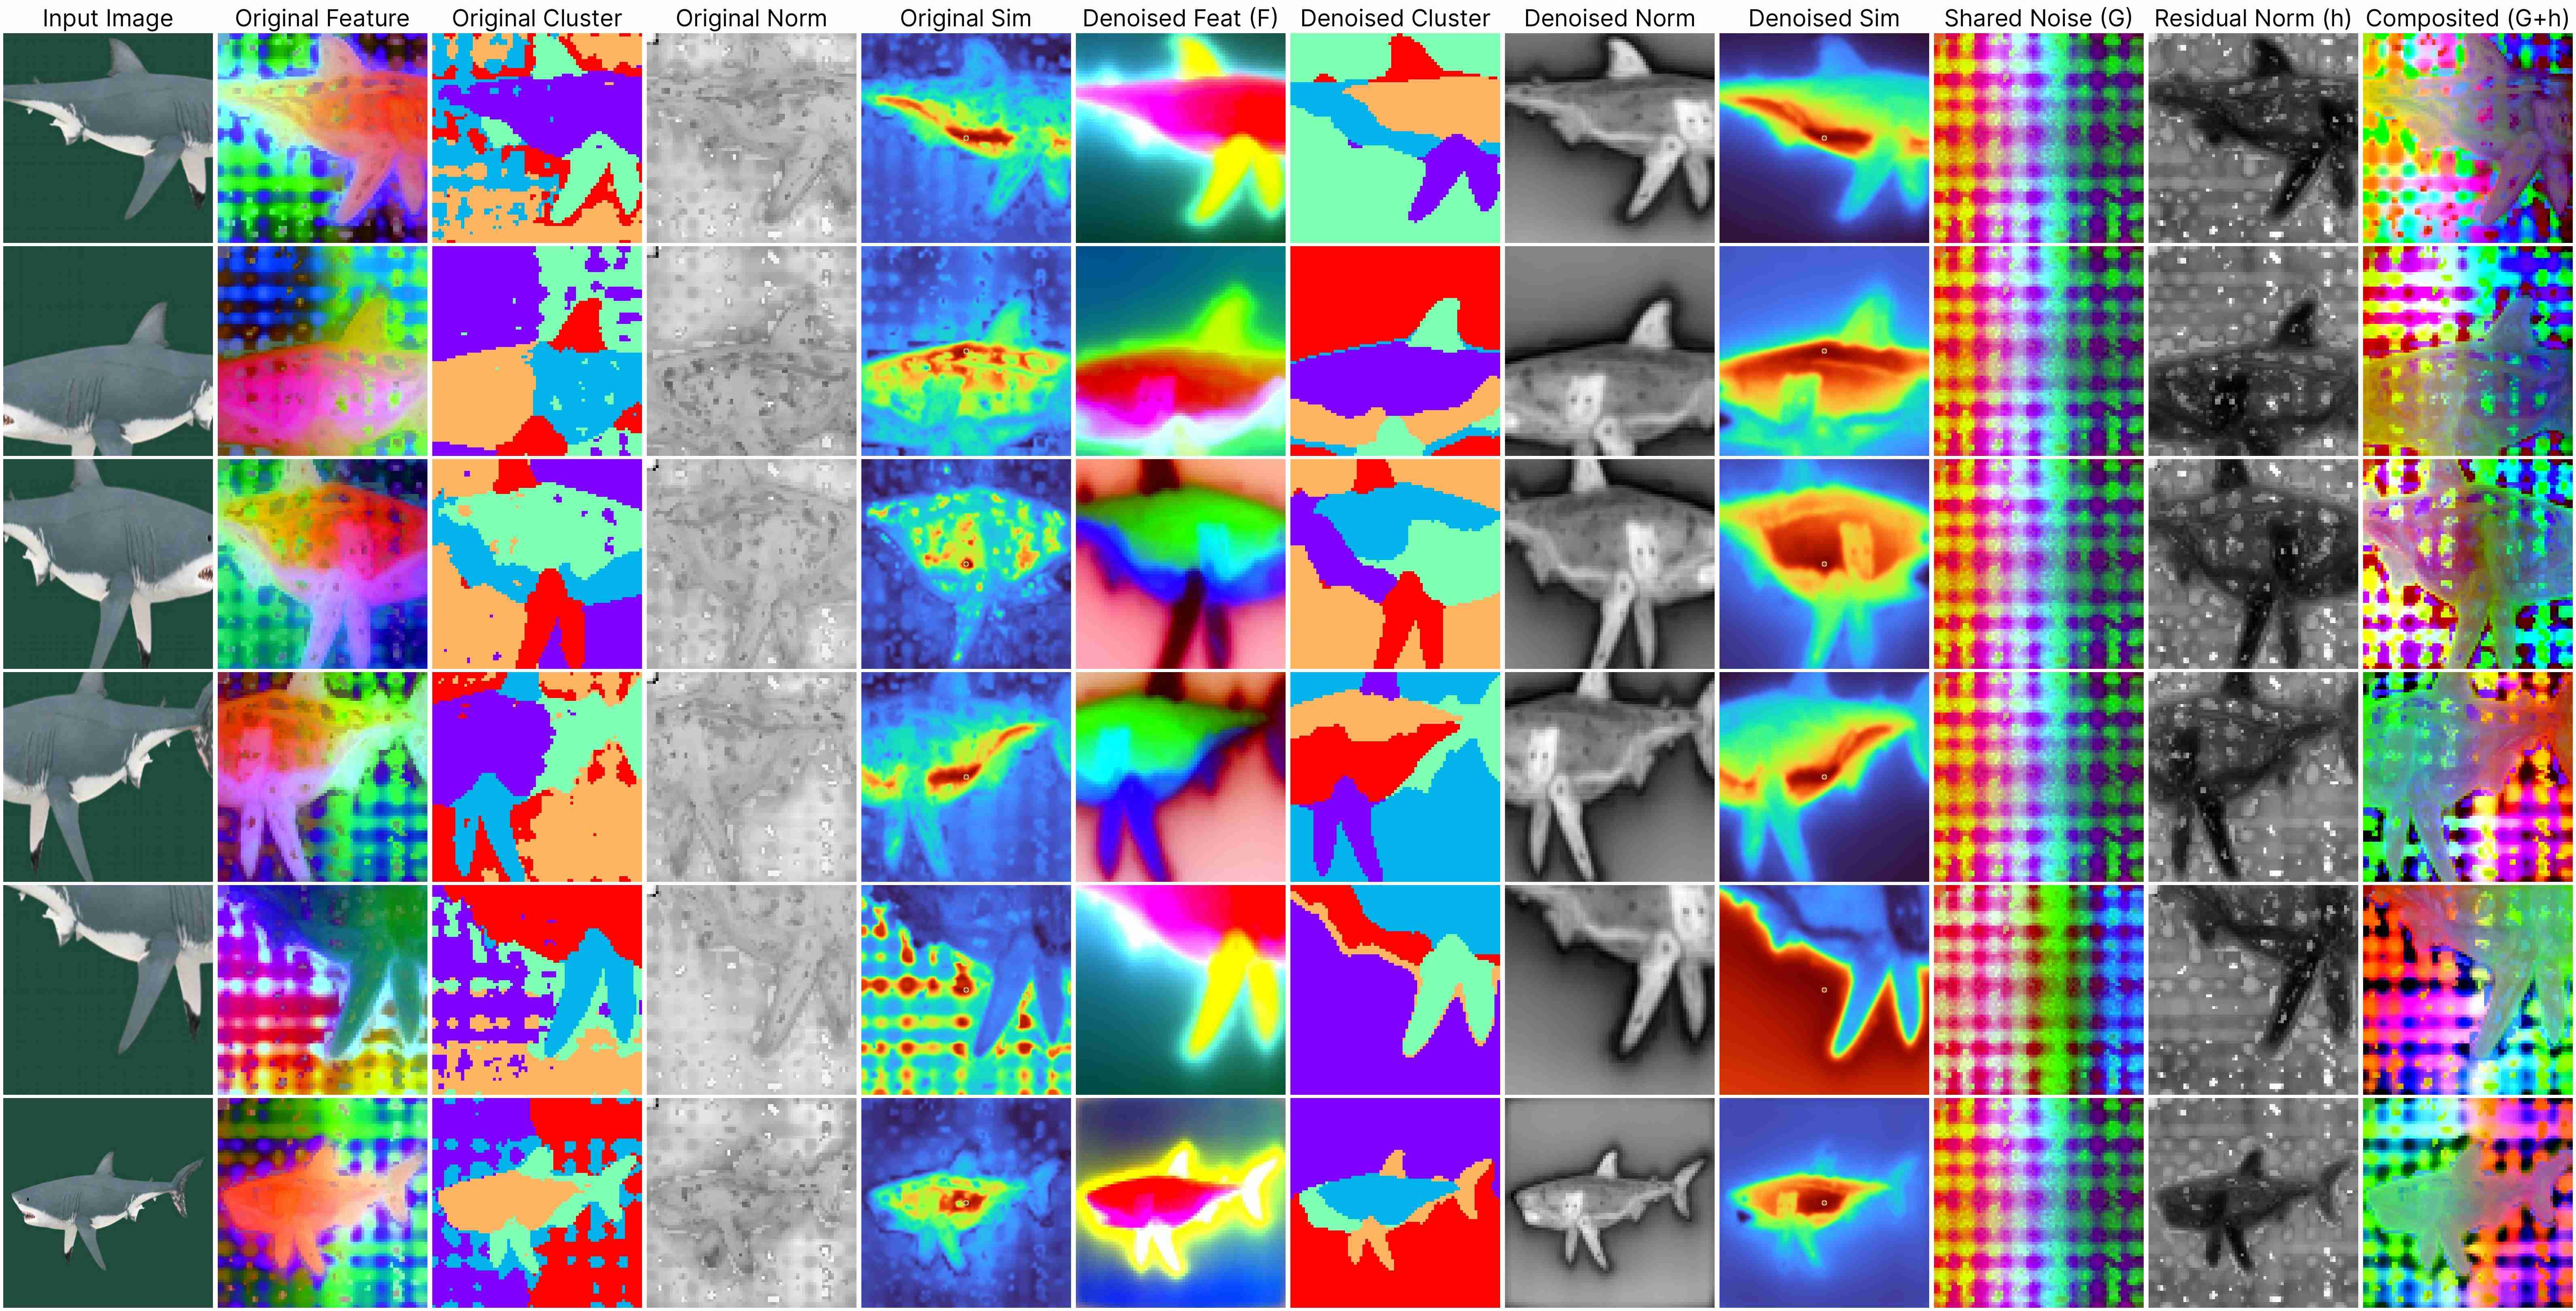
\includegraphics[width=\linewidth]{figures/per_img/vit_base_patch14_dinov2.lvd142m_stride7_n01491361_237.JPEG}
    \caption{\textbf{Visualization of DINOv2 \cite{oquab2023dinov2} per-image denoising}. We visualize all components of the per-image denoising stage. From left to right: In the first 5 columns we visualize the input image, the original noisy feature map from the model, the K-Means clusters on the original features, the L2 norm on the original features, and the similarity between the central red patch and other patches. In the next 4 columns we visualize the the denoised feature map using \ours{}, the denoised features' K-means clusters, the denoised features' L2 norms, and their similarity post-denoising. In the last 3 columns we visualize the decomposed shared noise term $\mathcal{G}$, the L2 norm of the predicted residual term $\vb{h}$, and the composite noise $(\mathcal{G} + \vb{h})$.}
    \label{fig:per_img_dinov2}
\end{figure}
%##################################################################################################
%##################################################################################################
\begin{figure}
    \centering
    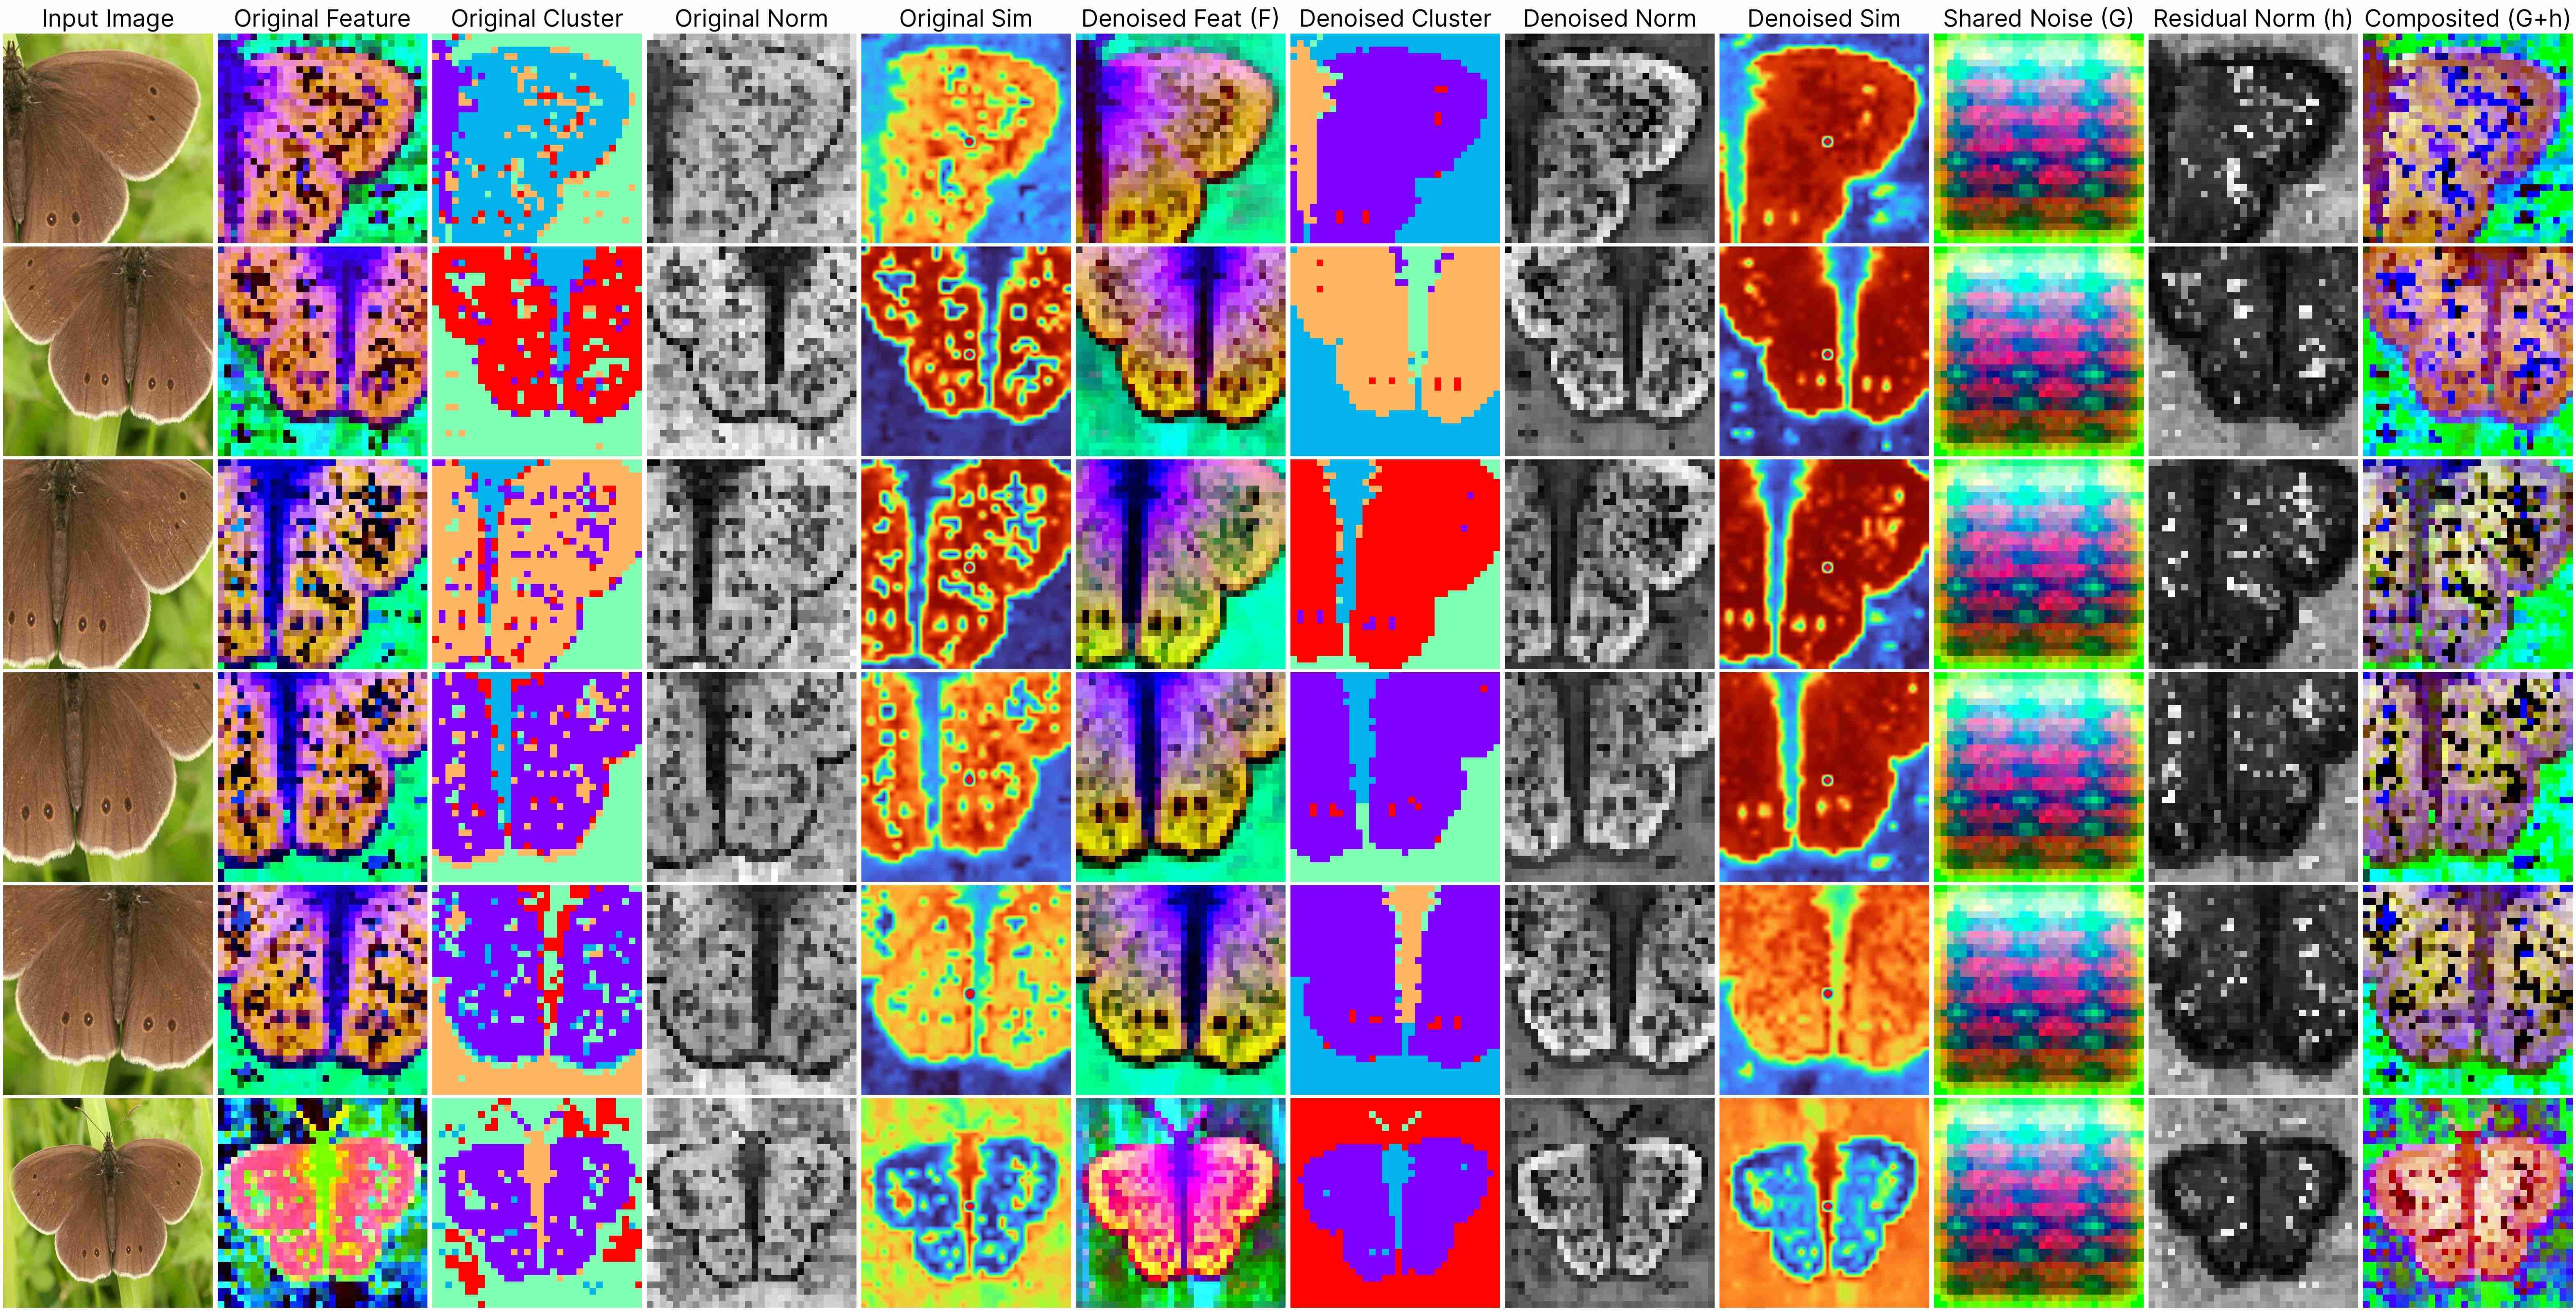
\includegraphics[width=\linewidth]{figures/per_img/vit_base_patch16_clip_384.laion2b_ft_in12k_in1k_stride16_n02277742_21913.JPEG}
    \caption{\textbf{Visualization of CLIP \cite{radford2021learning} per-image denoising}. We visualize all components of the per-image denoising stage. From left to right: In the first 5 columns we visualize the input image, the original noisy feature map from the model, the K-Means clusters on the original features, the L2 norm on the original features, and the similarity between the central red patch and other patches. In the next 4 columns we visualize the the denoised feature map using \ours{}, the denoised features' K-means clusters, the denoised features' L2 norms, and their similarity post-denoising. In the last 3 columns we visualize the decomposed shared noise term $\mathcal{G}$, the L2 norm of the predicted residual term $\vb{h}$, and the composite noise $(\mathcal{G} + \vb{h})$.}
    \label{fig:per_img_clip}
\end{figure}
%##################################################################################################
%##################################################################################################
\begin{figure}
    \centering
    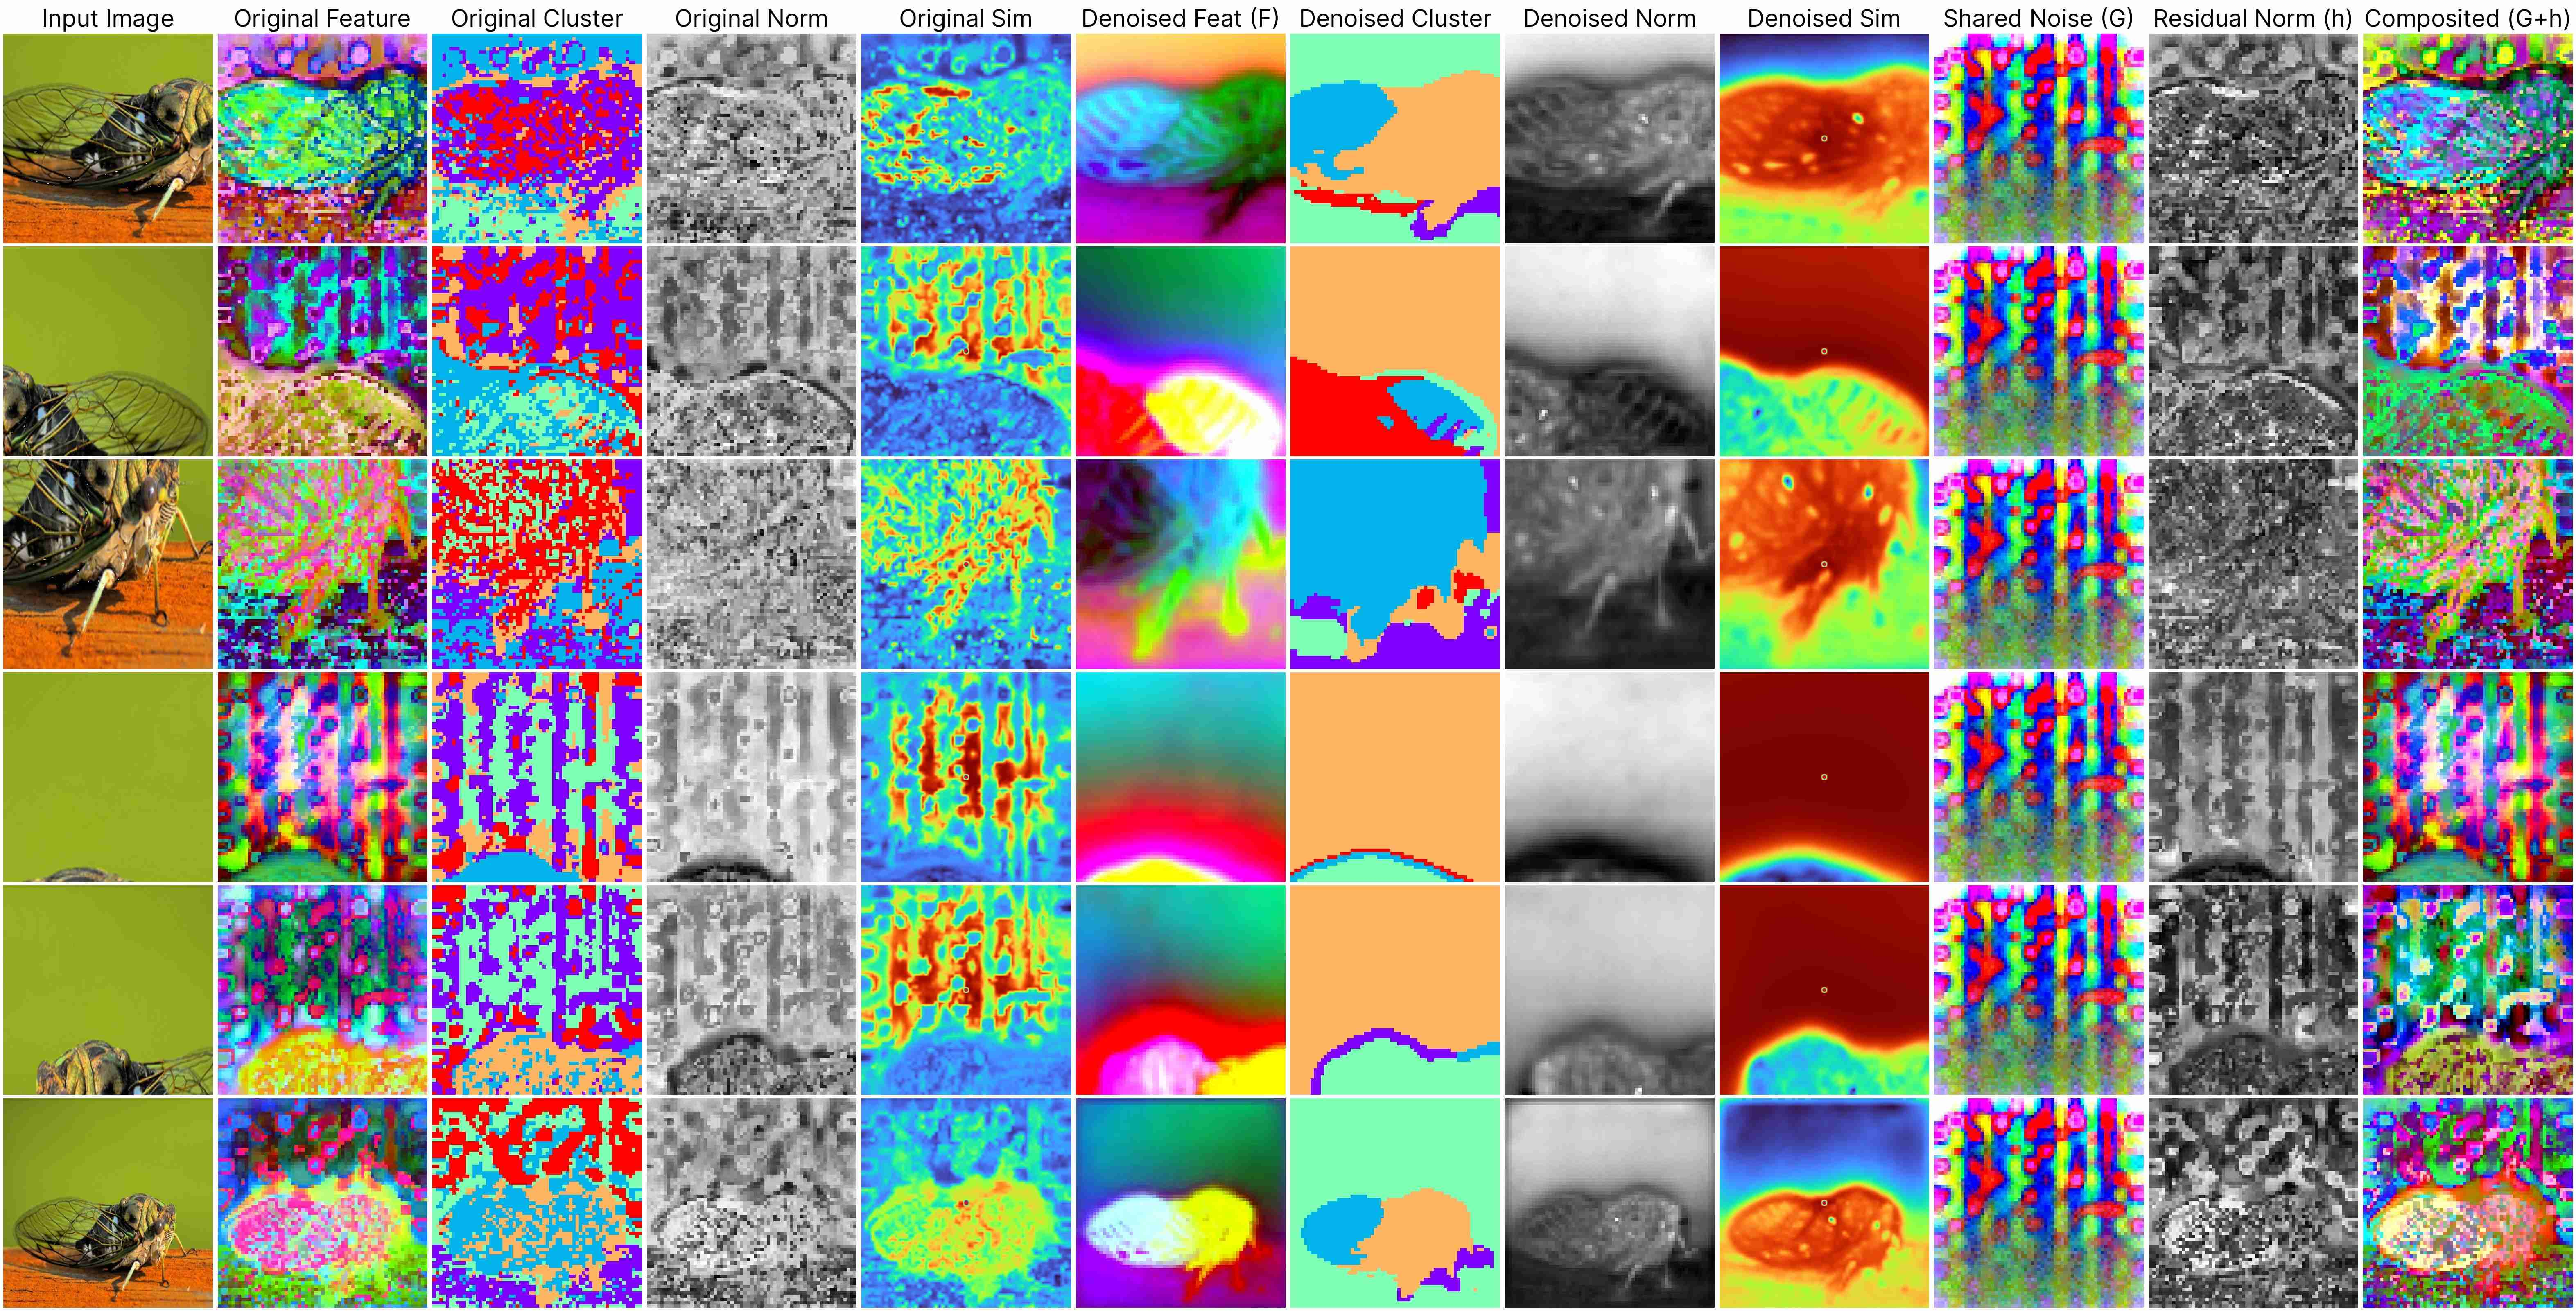
\includegraphics[width=\linewidth]{figures/per_img/eva02_base_patch16_clip_224.merged2b_stride8_n02256656_6922.JPEG}
    \caption{\textbf{Visualization of EVA02 \cite{fang2023eva} per-image denoising}. We visualize all components of the per-image denoising stage. From left to right: In the first 5 columns we visualize the input image, the original noisy feature map from the model, the K-Means clusters on the original features, the L2 norm on the original features, and the similarity between the central red patch and other patches. In the next 4 columns we visualize the the denoised feature map using \ours{}, the denoised features' K-means clusters, the denoised features' L2 norms, and their similarity post-denoising. In the last 3 columns we visualize the decomposed shared noise term $\mathcal{G}$, the L2 norm of the predicted residual term $\vb{h}$, and the composite noise $(\mathcal{G} + \vb{h})$.}
    \label{fig:per_img_eva}
\end{figure}
%##################################################################################################
%##################################################################################################
\begin{figure}
    \centering
    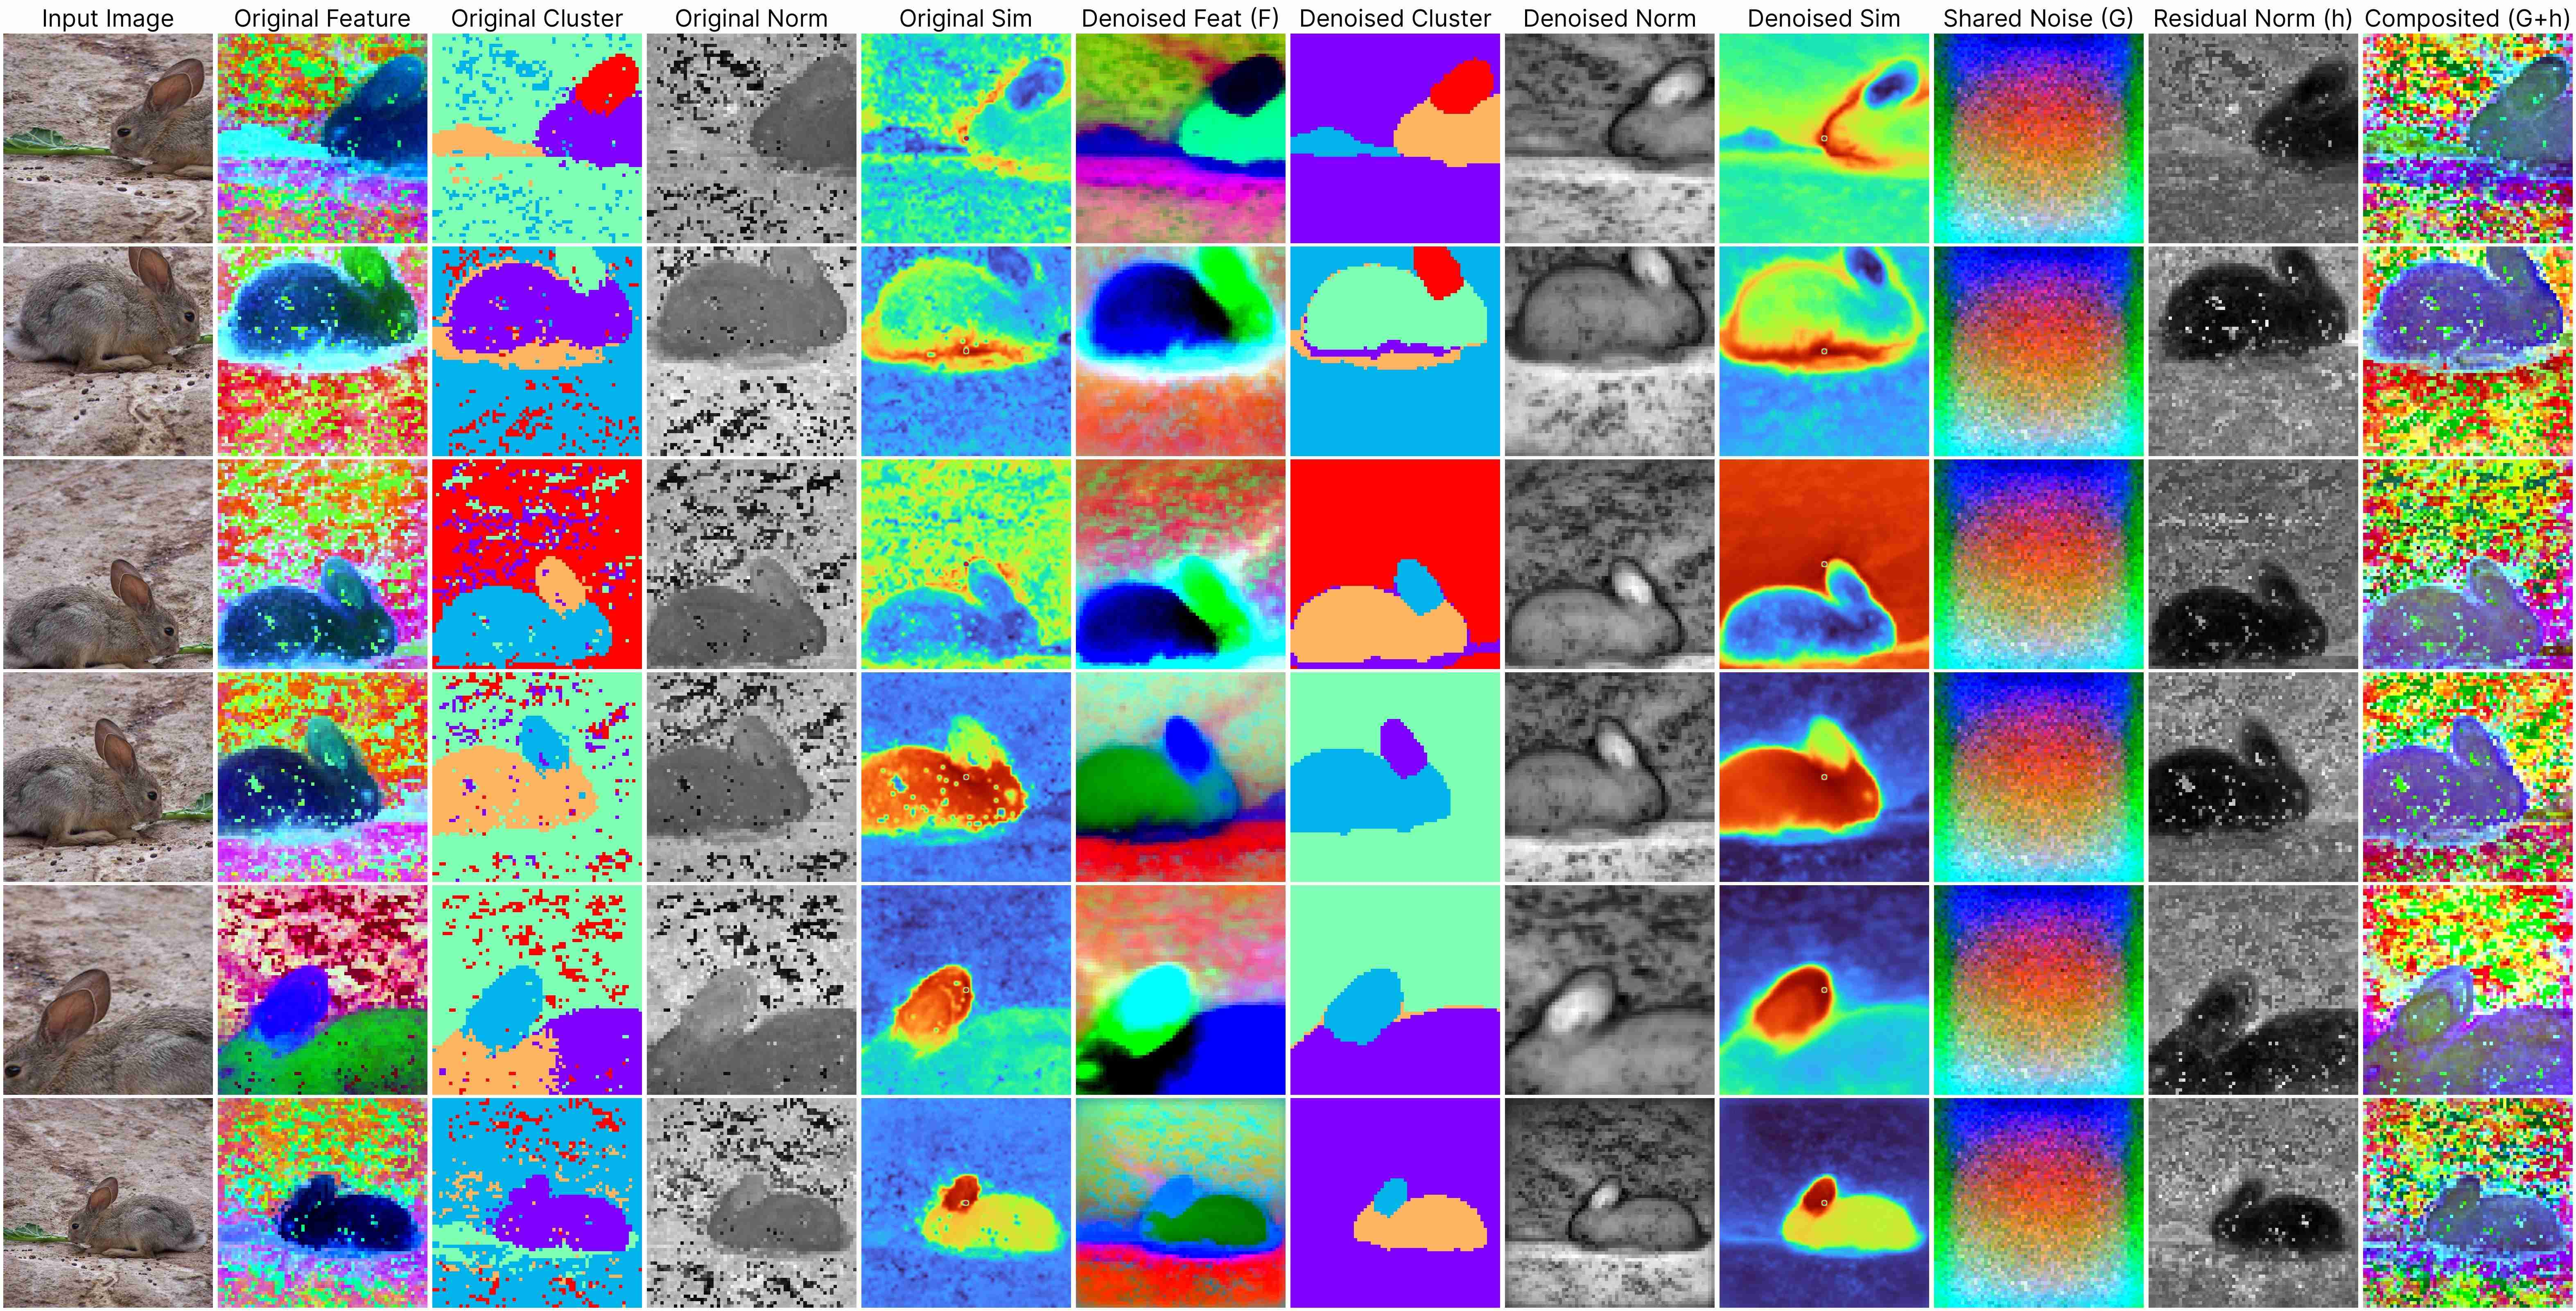
\includegraphics[width=\linewidth]{figures/per_img/deit3_base_patch16_224.fb_in1k_stride8_n02325366_1544.JPEG}
    \caption{\textbf{Visualization of DeiT-III \cite{touvron2022deit} per-image denoising}. We visualize all components of the per-image denoising stage. From left to right: In the first 5 columns we visualize the input image, the original noisy feature map from the model, the K-Means clusters on the original features, the L2 norm on the original features, and the similarity between the central red patch and other patches. In the next 4 columns we visualize the the denoised feature map using \ours{}, the denoised features' K-means clusters, the denoised features' L2 norms, and their similarity post-denoising. In the last 3 columns we visualize the decomposed shared noise term $\mathcal{G}$, the L2 norm of the predicted residual term $\vb{h}$, and the composite noise $(\mathcal{G} + \vb{h})$.}
    \label{fig:per_img_deit}
\end{figure}
%##################################################################################################
%##################################################################################################
\begin{figure}
    \centering
    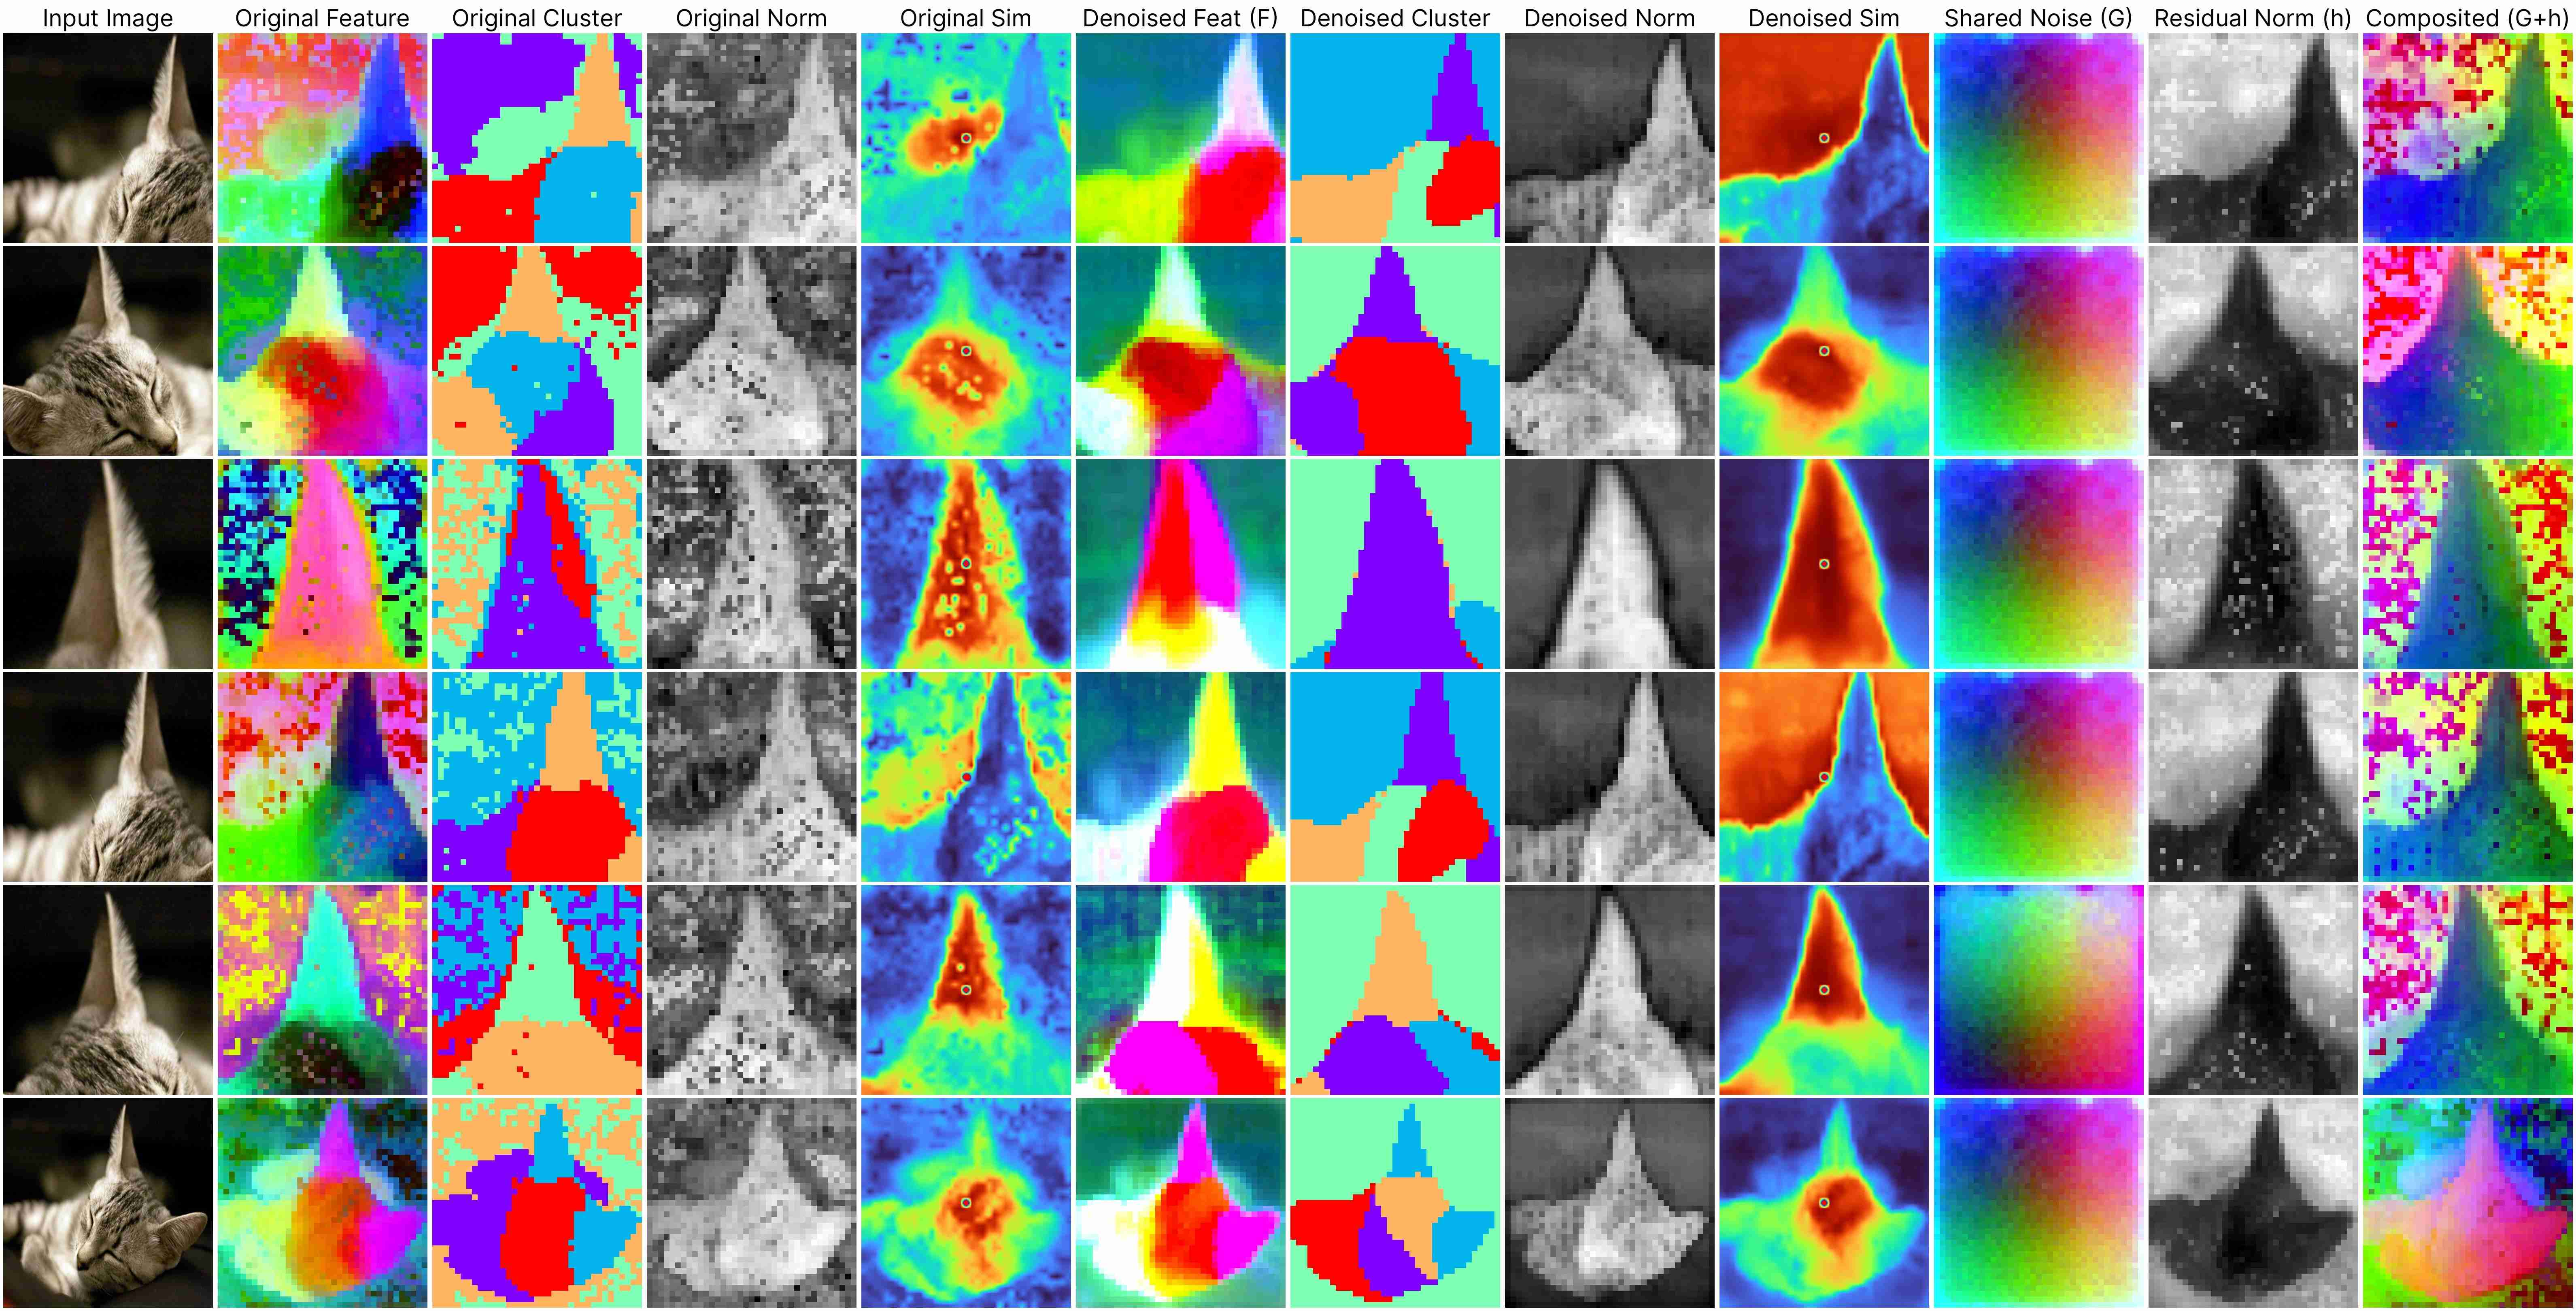
\includegraphics[width=\linewidth]{figures/per_img/vit_base_patch14_reg4_dinov2.lvd142m_stride14_n02124075_7651.JPEG}
    \caption{\textbf{Visualization of DINOv2 with Registers \cite{darcet2023vision} per-image denoising}. We visualize all components of the per-image denoising stage. From left to right: In the first 5 columns we visualize the input image, the original noisy feature map from the model, the K-Means clusters on the original features, the L2 norm on the original features, and the similarity between the central red patch and other patches. In the next 4 columns we visualize the the denoised feature map using \ours{}, the denoised features' K-means clusters, the denoised features' L2 norms, and their similarity post-denoising. In the last 3 columns we visualize the decomposed shared noise term $\mathcal{G}$, the L2 norm of the predicted residual term $\vb{h}$, and the composite noise $(\mathcal{G} + \vb{h})$.}
    \label{fig:per_img_register}
\end{figure}
%##################################################################################################

%##################################################################################################
\begin{figure}
    \centering
    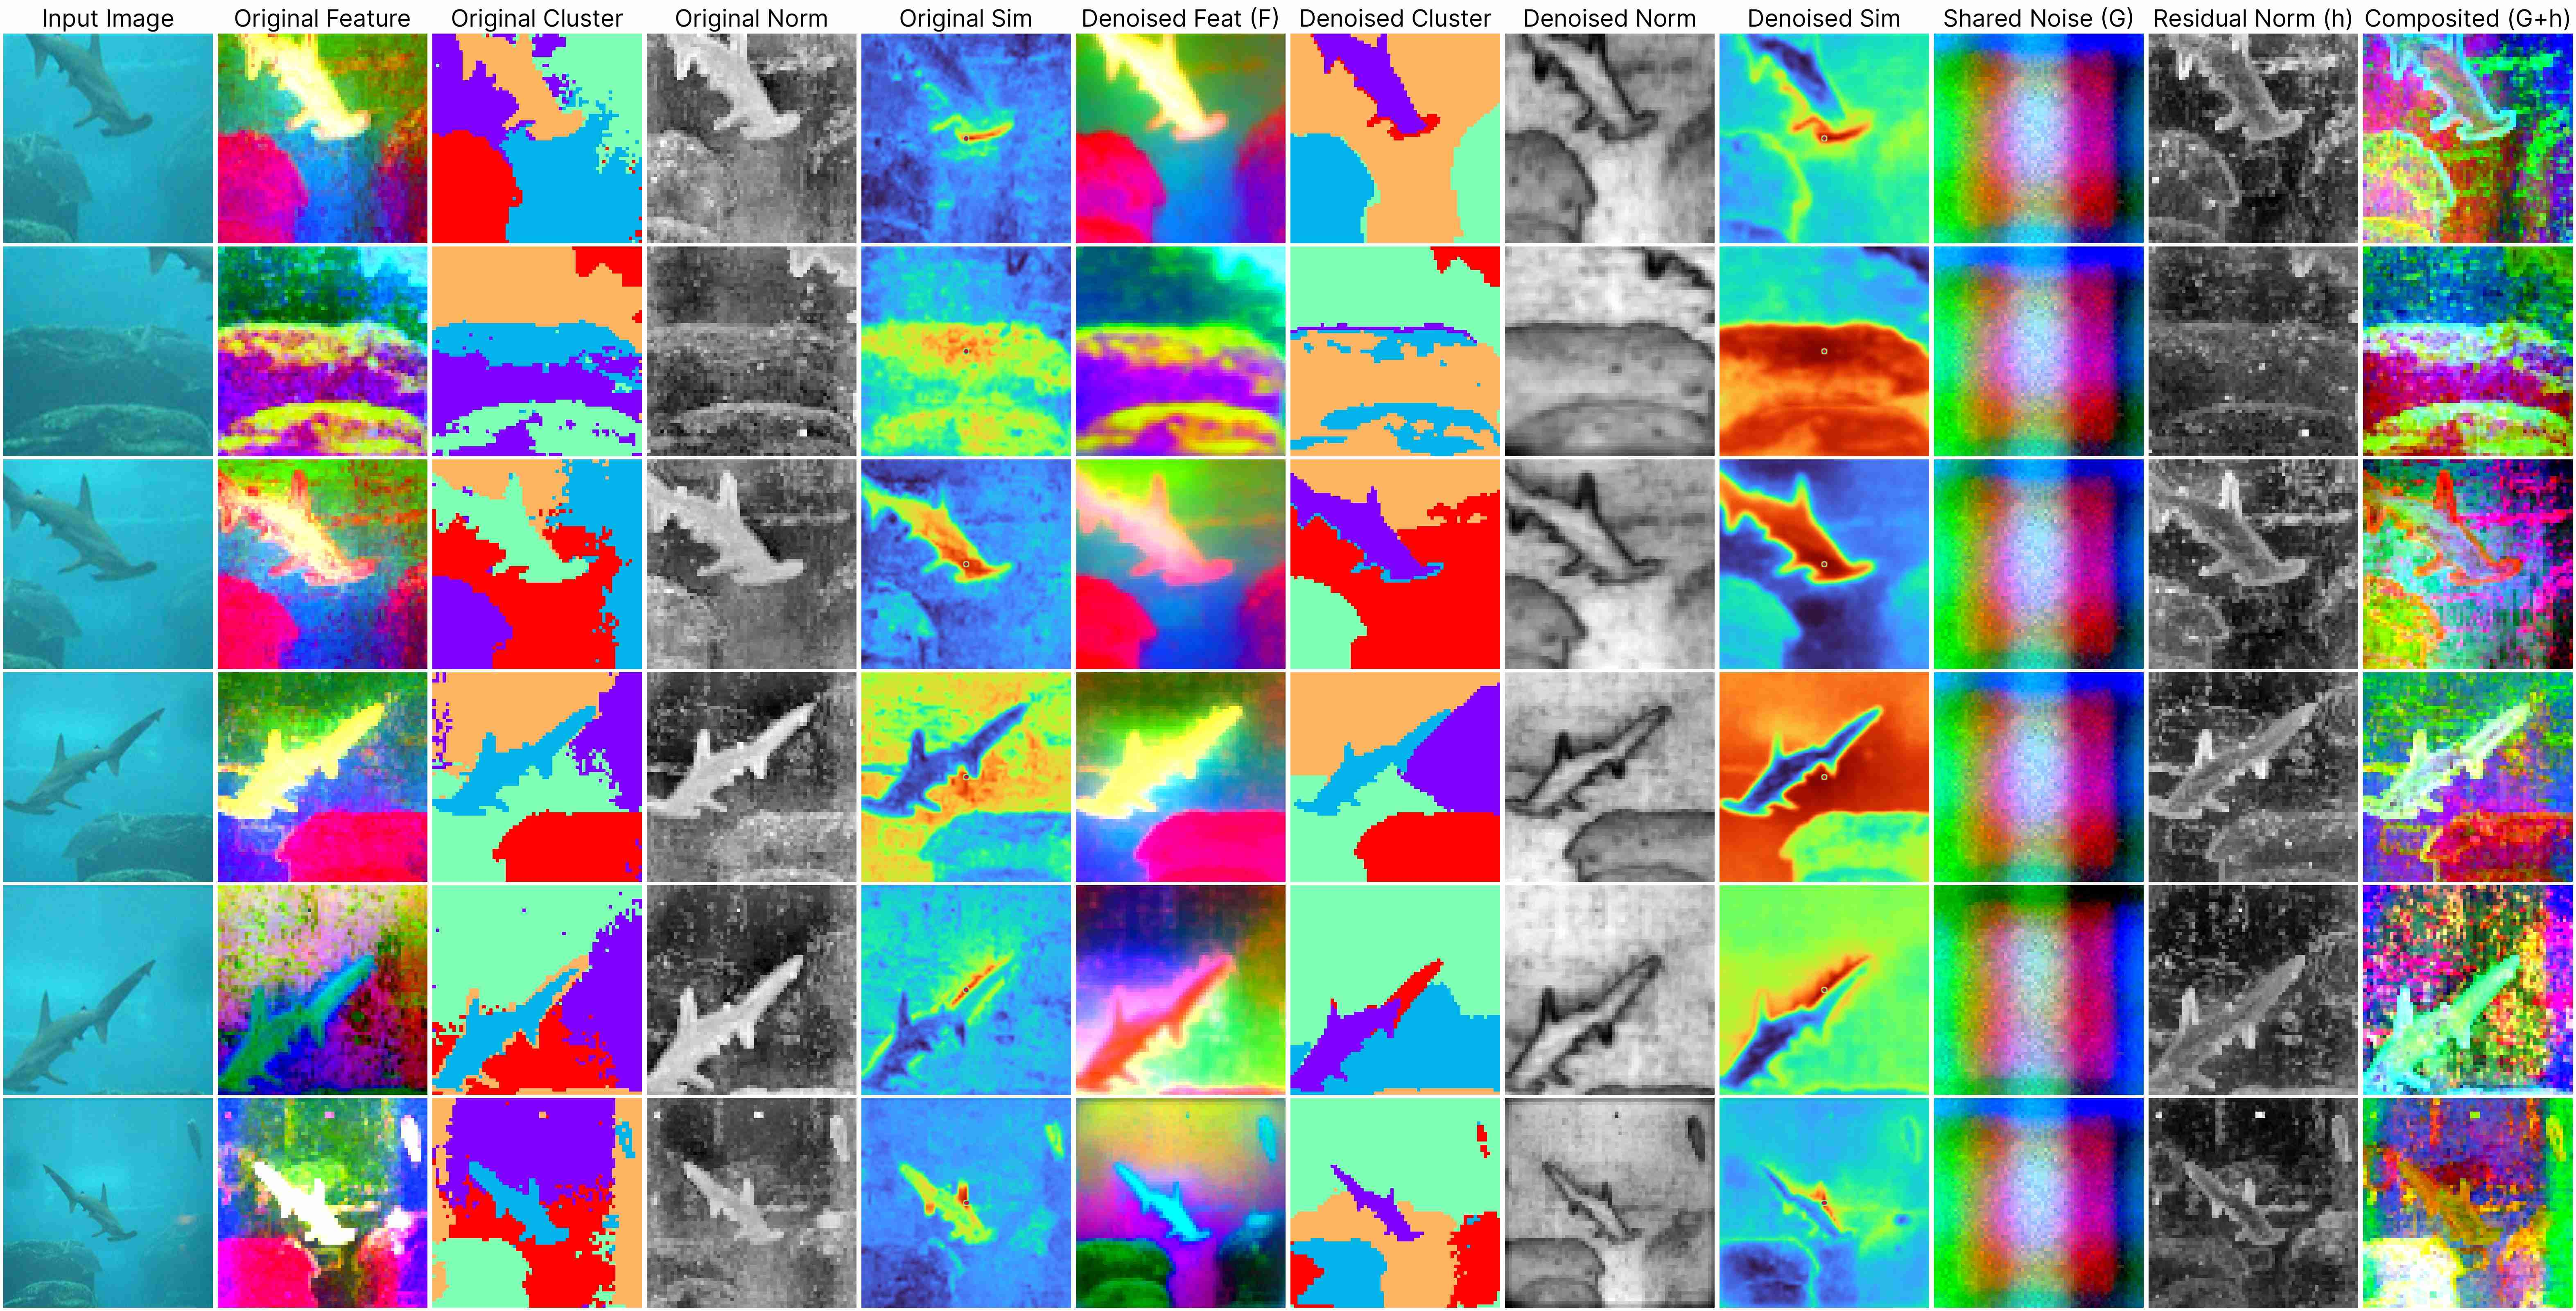
\includegraphics[width=\linewidth]{figures/per_img/vit_base_patch16_224.dino_stride8_n01494475_3981.JPEG}
    \caption{\textbf{Visualization of DINO \cite{caron2021emerging} per-image denoising}. We visualize all components of the per-image denoising stage. From left to right: In the first 5 columns we visualize the input image, the original noisy feature map from the model, the K-Means clusters on the original features, the L2 norm on the original features, and the similarity between the central red patch and other patches. In the next 4 columns we visualize the the denoised feature map using \ours{}, the denoised features' K-means clusters, the denoised features' L2 norms, and their similarity post-denoising. In the last 3 columns we visualize the decomposed shared noise term $\mathcal{G}$, the L2 norm of the predicted residual term $\vb{h}$, and the composite noise $(\mathcal{G} + \vb{h})$.}
    \label{fig:per_img_dino}
\end{figure}
%##################################################################################################

%##################################################################################################
\begin{figure}
    \centering
    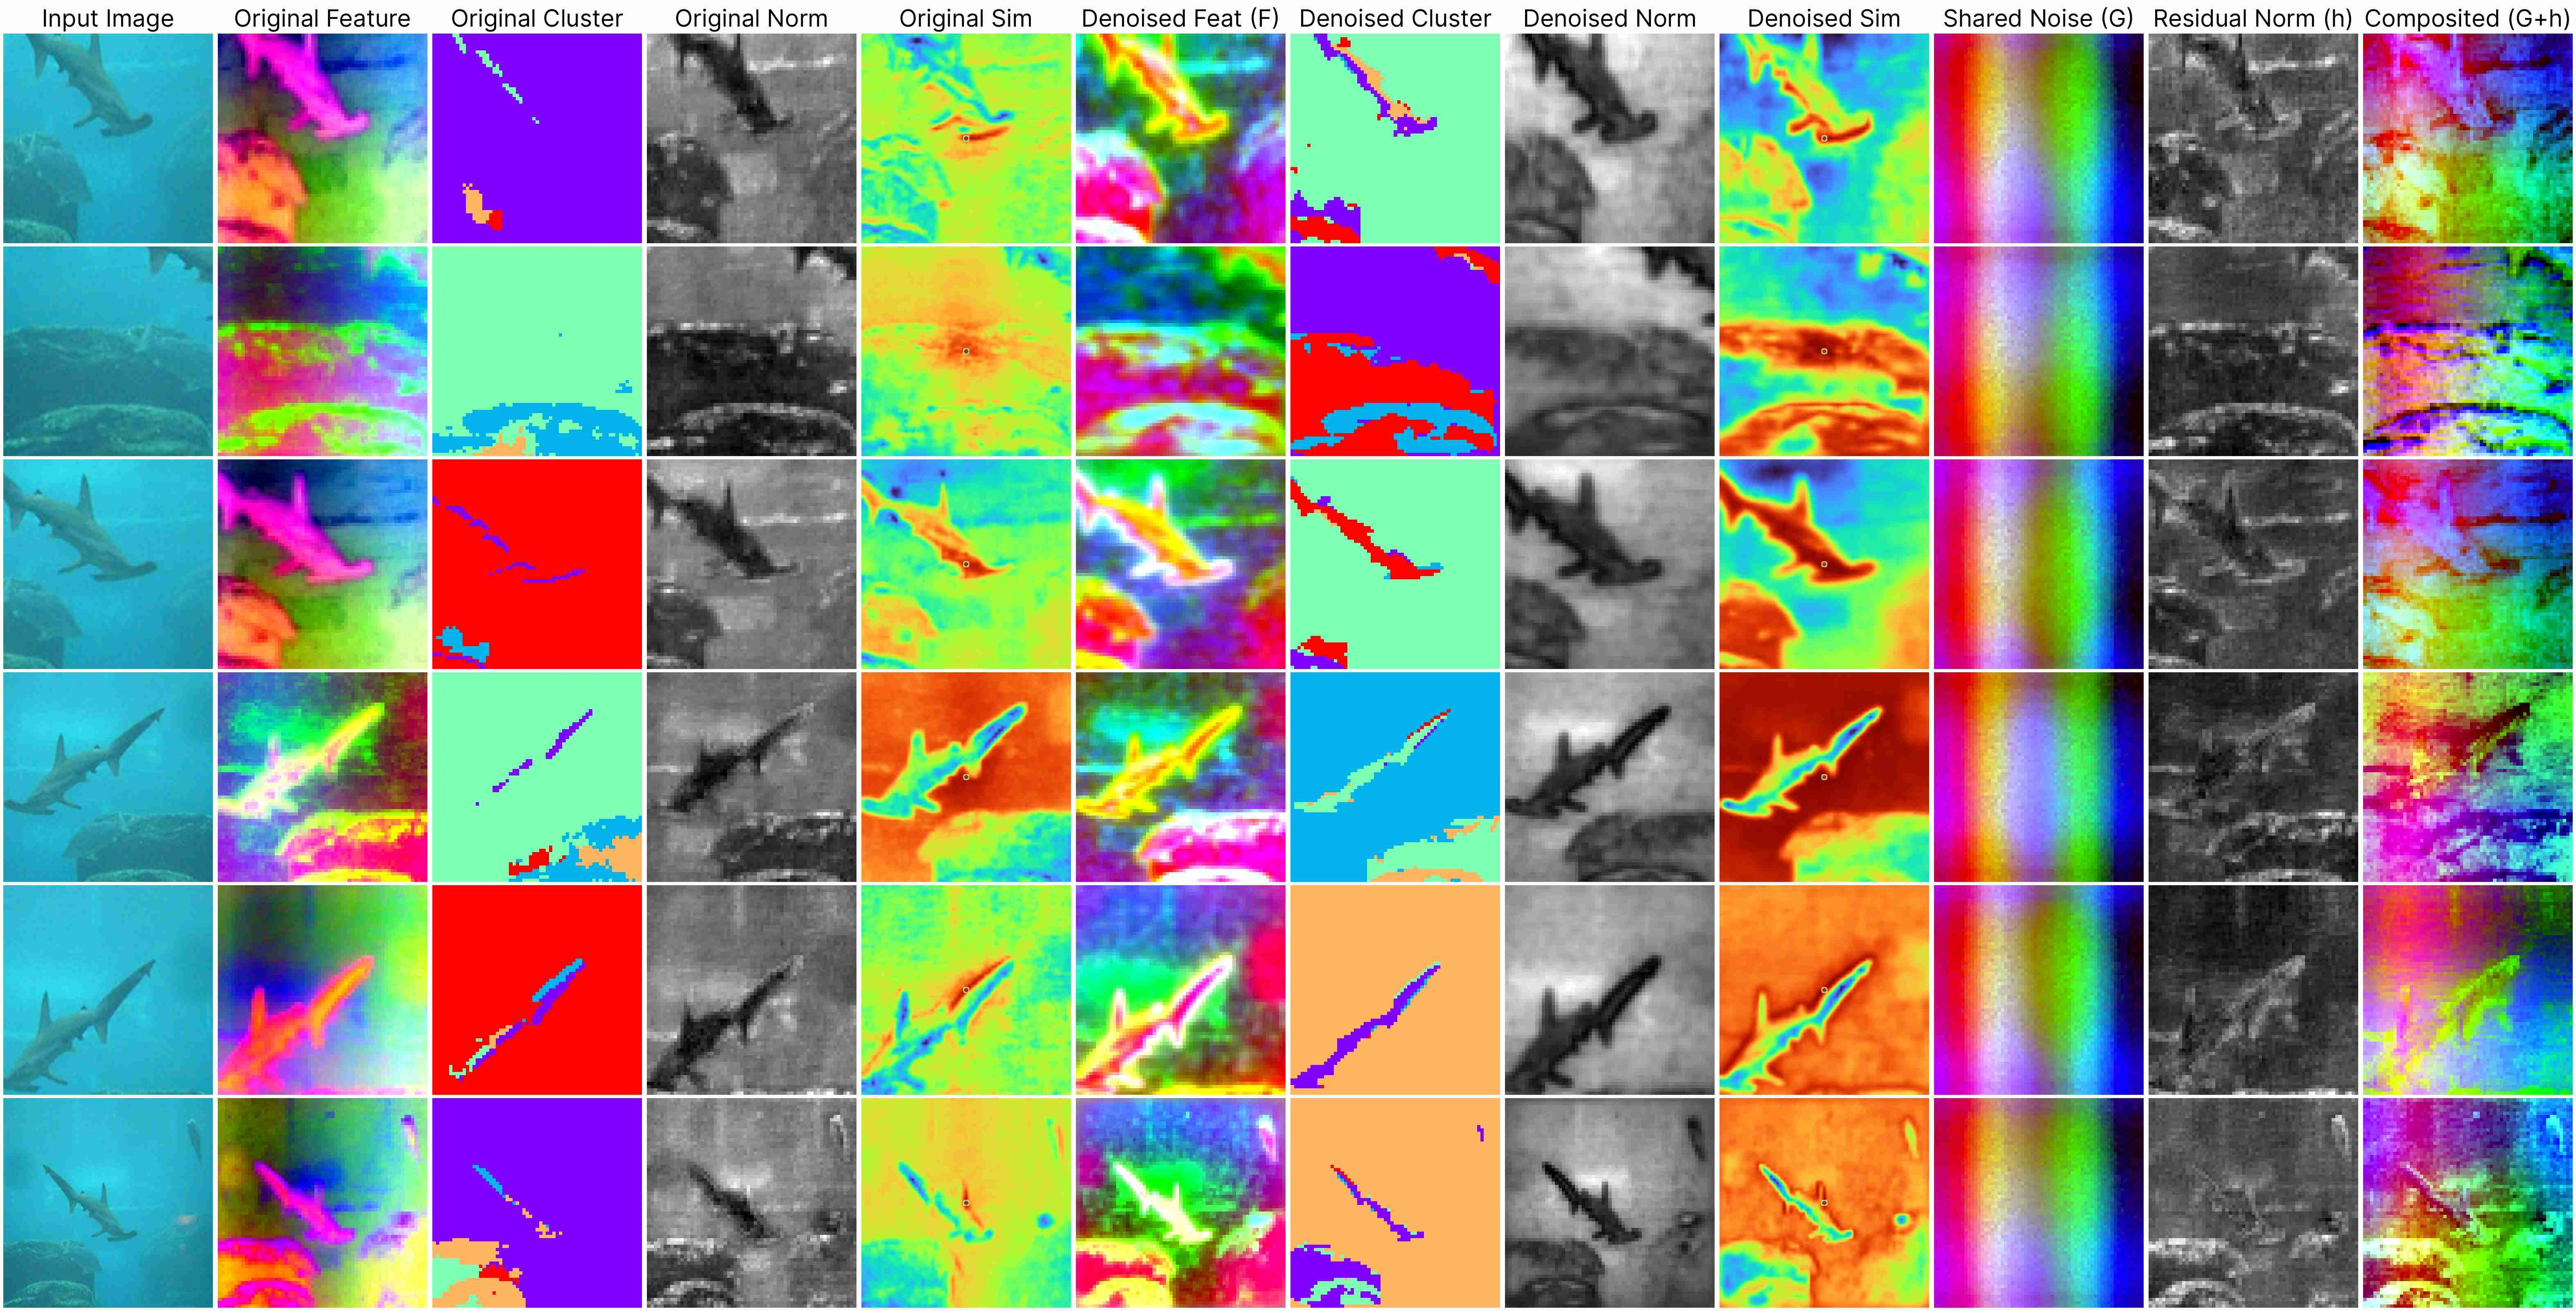
\includegraphics[width=\linewidth]{figures/per_img/vit_base_patch16_224.mae_stride8_n01494475_3981.JPEG}
    \caption{\textbf{Visualization of MAE \cite{he2022masked} per-image denoising}. We visualize all components of the per-image denoising stage. From left to right: In the first 5 columns we visualize the input image, the original noisy feature map from the model, the K-Means clusters on the original features, the L2 norm on the original features, and the similarity between the central red patch and other patches. In the next 4 columns we visualize the the denoised feature map using \ours{}, the denoised features' K-means clusters, the denoised features' L2 norms, and their similarity post-denoising. In the last 3 columns we visualize the decomposed shared noise term $\mathcal{G}$, the L2 norm of the predicted residual term $\vb{h}$, and the composite noise $(\mathcal{G} + \vb{h})$.}
    \label{fig:per_img_mae}
\end{figure}
%##################################################################################################


\section{Discussion on Limitations}
\label{sec:limitation}
\paragraph{Limitations.} Our approach faces some practical and theoretical challenges. On the practical front, although our method leverages parallel computing to amortize the denoising process, the time required to denoise a single image, such as one with a resolution of $518 \times 518$, remains high --- approximately 100 seconds. This duration may be impractical for commercial or personal users with limited access to parallel computing resources, despite the fact that we can finish denoising 10k samples within hours. Additionally, our generalizable denoisesr, trained on the last layer features of pretrained ViTs, does not remove noise in intermediate outputs. Users requiring denoised features from multiple layers might need to train distinct denoisers for different layers. From the theoretical perspective, the reasons behind the presence of these artifacts remain unclear. Integrating insights from Registers \cite{darcet2023vision} with our findings could yield a more comprehensive understanding of these phenomena.

\paragraph{Broader Impact.} Our work serves as one of the initial studies to understand the position-based artifacts present in the features of ViT models. We identify and propose methods to mitigate these artifacts, yet the root causes and characteristics of these artifacts are not fully understood. The severity of artifacts varies with the training algorithms; for instance, DINOv2 exhibits more pronounced artifacts compared to MAE, which shows subtler discrepancies.
Thus, one direction of exploration is to investigate the training paradigm that includes supervision ---\ie local \vs global --- as well as the loss-induced parameter landscape ---\ie sharp \vs smooth Hessians.
Furthermore, a better architectural design---\eg new positional embeddings---may diminish the severity of the feature artifacts. In this work, we do not explore modifying the ViT's design; however, more study into its positional embeddings and the effect on downstream features should prove interesting.
Ultimately, we believe our findings are intriguing to the community and more research is needed to better understand this fundamental problem.
